% !TEX root=./adl.tex

% Flash Attention color palette
\definecolor{fagreen}{RGB}{34, 139, 34}
\definecolor{fablue}{RGB}{30, 100, 200}
\definecolor{fared}{RGB}{180, 40, 40}
\definecolor{fagray}{RGB}{90, 90, 90}
\definecolor{fasram}{RGB}{255, 180, 50}
\definecolor{fahbm}{RGB}{100, 160, 220}
\definecolor{barblue}{RGB}{99, 135, 177}
\definecolor{baredge}{RGB}{30, 30, 60}
\definecolor{sramcol}{RGB}{232, 126, 50}
\definecolor{hbmcol}{RGB}{105, 165, 110}
\definecolor{dramcol}{RGB}{120, 185, 175}
\definecolor{pyredge}{RGB}{20, 20, 20}

\lstset{
  language=Python,
  basicstyle=\tiny\ttfamily,
  keywordstyle=\color{fablue}\bfseries,
  commentstyle=\color{fagray},
  stringstyle=\color{fagreen},
  showstringspaces=false,
  frame=single,
  rulecolor=\color{fagray!40},
  xleftmargin=0.5em,
  xrightmargin=0.5em,
}

% -----------------------------------------------------------------------
\section{Flash Attention}\label{ch:flash}

% -----------------------------------------------------------------------
\begin{frame}{Flash Attention: Overview}

  \begin{block}{Acknowledgements}
    {\footnotesize Materials based on Umar Jamil's lecture \cite{jamil2024flashattention} and repository \cite{jamil2024tritonflash}.}
  \end{block}

  \begin{description}
    \item[What] Exact attention, reformulated to match the GPU memory hierarchy. Same outputs, much faster, linear memory.
    \item[Why] Standard kernel in modern transformers; canonical example of algorithm/hardware co-design.
    \item[Topics]
      \begin{itemize}
        \item GPU memory hierarchy, online softmax.
        \item Forward and backward pass.
        \item GPU programming: CUDA, Triton, tiled matmul.
        \item Flash Attention in Triton with PyTorch autograd.
      \end{itemize}
  \end{description}
\end{frame}

% -----------------------------------------------------------------------
\begin{frame}{The Problem with Standard Attention}

  Recall: $\text{Attn}(Q,K,V) = \text{softmax}\!\left(\frac{QK^\top}{\sqrt{d}}\right) V$

  \vspace{0.2em}
  \begin{columns}
    \begin{column}{0.55\textwidth}
      \textbf{The bottleneck is \emph{not} arithmetic}, it is \textbf{memory}:
      \begin{itemize}
        \item The $T \times T$ matrix $S = QK^\top$ must be materialized in HBM
        \item Writing $S$ to HBM and reading it back dominates wall-clock time
      \end{itemize}

      \begin{alertblock}{Memory-bound, not compute-bound}
        Standard attention spends most time on memory transfers, not on FLOPs.
      \end{alertblock}

      {\small \cite{dao2022flashattention} \quad \cite{dao2023flashattention2} \quad \cite{jamil2024flashattention}}
    \end{column}
    \begin{column}{0.42\textwidth}
      \centering
      \resizebox{\linewidth}{!}{%
      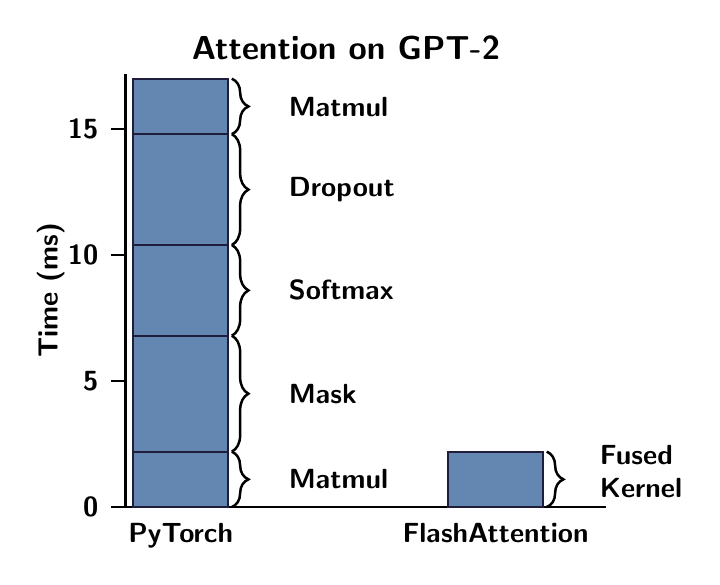
\begin{tikzpicture}[
          font=\sffamily,
          seg/.style={draw=baredge, line width=0.7pt, fill=barblue},
          brace/.style={decorate, decoration={brace, amplitude=6pt, raise=0pt, mirror}, line width=0.9pt},
          lab/.style={font=\sffamily\bfseries, anchor=west},
        ]
        \def\barx{0}
        \def\barxR{4.0}
        \def\barw{1.2}
        \def\unit{0.32}
        \pgfmathsetmacro{\yMax}{17.2*\unit}

        % y axis
        \draw[line width=1pt] (-0.1,0) -- (-0.1,\yMax);
        \foreach \v in {0,5,10,15} {
          \draw[line width=1pt] (-0.28,{\v*\unit}) -- (-0.1,{\v*\unit});
          \node[anchor=east, font=\sffamily\bfseries] at (-0.32,{\v*\unit}) {\v};
        }
        \node[rotate=90, font=\sffamily\bfseries] at (-1.05, {\yMax/2}) {Time (ms)};

        % x axis
        \draw[line width=1pt] (-0.1,0) -- (6.0,0);

        % title
        \node[font=\sffamily\bfseries\large, anchor=south] at (2.7, {\yMax+0.05}) {Attention on GPT-2};

        % left bar segments (heights in ms)
        \def\hMatA{2.2}
        \def\hMask{4.6}
        \def\hSoft{3.6}
        \def\hDrop{4.4}
        \def\hMatB{2.2}
        \pgfmathsetmacro{\yA}{\hMatA}
        \pgfmathsetmacro{\yB}{\yA+\hMask}
        \pgfmathsetmacro{\yC}{\yB+\hSoft}
        \pgfmathsetmacro{\yD}{\yC+\hDrop}
        \pgfmathsetmacro{\yE}{\yD+\hMatB}
        \draw[seg] (\barx,0) rectangle ({\barx+\barw},{\yA*\unit});
        \draw[seg] (\barx,{\yA*\unit}) rectangle ({\barx+\barw},{\yB*\unit});
        \draw[seg] (\barx,{\yB*\unit}) rectangle ({\barx+\barw},{\yC*\unit});
        \draw[seg] (\barx,{\yC*\unit}) rectangle ({\barx+\barw},{\yD*\unit});
        \draw[seg] (\barx,{\yD*\unit}) rectangle ({\barx+\barw},{\yE*\unit});

        % braces and labels
        \def\bex{\barx+\barw+0.05}
        \def\bx{1.85}
        \draw[brace] ({\bex},{0*\unit}) -- ({\bex},{\yA*\unit});
        \node[lab] at (\bx,{(\yA/2)*\unit}) {Matmul};
        \draw[brace] ({\bex},{\yA*\unit}) -- ({\bex},{\yB*\unit});
        \node[lab] at (\bx,{((\yA+\yB)/2)*\unit}) {Mask};
        \draw[brace] ({\bex},{\yB*\unit}) -- ({\bex},{\yC*\unit});
        \node[lab] at (\bx,{((\yB+\yC)/2)*\unit}) {Softmax};
        \draw[brace] ({\bex},{\yC*\unit}) -- ({\bex},{\yD*\unit});
        \node[lab] at (\bx,{((\yC+\yD)/2)*\unit}) {Dropout};
        \draw[brace] ({\bex},{\yD*\unit}) -- ({\bex},{\yE*\unit});
        \node[lab] at (\bx,{((\yD+\yE)/2)*\unit}) {Matmul};

        % right bar
        \def\hFused{2.2}
        \draw[seg] (\barxR,0) rectangle ({\barxR+\barw},{\hFused*\unit});
        \draw[brace] ({\barxR+\barw+0.05},{0*\unit}) -- ({\barxR+\barw+0.05},{\hFused*\unit});
        \node[lab, align=left] at ({\barxR+\barw+0.6},{(\hFused/2)*\unit + 0.1}) {Fused\\Kernel};

        % x labels
        \node[font=\sffamily\bfseries, anchor=north] at ({\barx+\barw/2},-0.08) {PyTorch};
        \node[font=\sffamily\bfseries, anchor=north] at ({\barxR+\barw/2},-0.08) {FlashAttention};
      \end{tikzpicture}}
    \end{column}
  \end{columns}
\end{frame}

% -----------------------------------------------------------------------
\subsection{Motivation \& GPU Memory Hierarchy}

\begin{frame}{HBM vs.\ SRAM}

  \begin{columns}
    \begin{column}{0.55\textwidth}
      GPUs have a two-level memory hierarchy:

      \vspace{0.5em}
      \begin{description}
        \item[HBM (off-chip):] Stores model parameters, activations, optimizer states. Every kernel reads inputs from and writes outputs to HBM.
        \item[SRAM (on-chip):] Each streaming multiprocessor has its own SRAM (shared memory). Data must be explicitly loaded into SRAM before compute.
      \end{description}

      \vspace{0.5em}
      \begin{alertblock}{Implication for attention}
        Standard attention writes $S, P \in \mathbb{R}^{T \times T}$ to HBM between steps. Flash attention computes $S$ and $P$ block-wise in SRAM on-the-fly, avoiding the HBM round-trip.
      \end{alertblock}
    \end{column}
    \begin{column}{0.42\textwidth}
      \centering
      \resizebox{\linewidth}{!}{%
      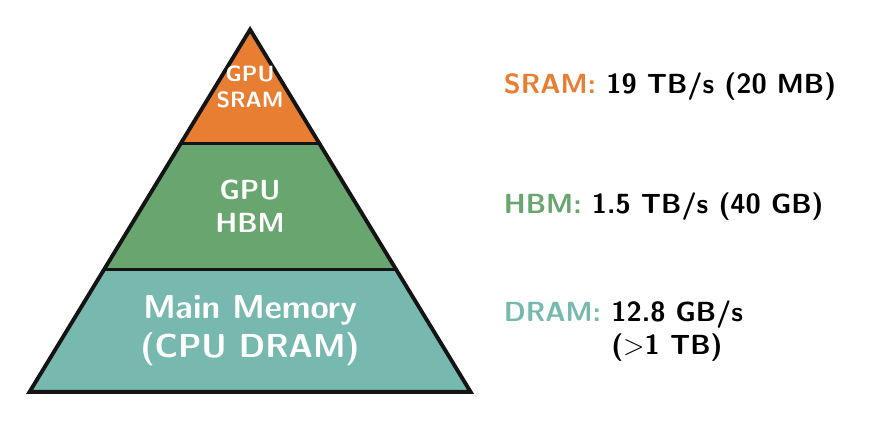
\begin{tikzpicture}[font=\sffamily\bfseries]
        \def\H{4.6}
        \def\W{2.8}
        \def\yA{3.15}
        \def\yB{1.55}
        \pgfmathsetmacro{\xA}{(1-\yA/\H)*\W}
        \pgfmathsetmacro{\xB}{(1-\yB/\H)*\W}

        % Slices
        \fill[sramcol] (0,\H) -- (\xA,\yA) -- (-\xA,\yA) -- cycle;
        \fill[hbmcol] (-\xA,\yA) -- (\xA,\yA) -- (\xB,\yB) -- (-\xB,\yB) -- cycle;
        \fill[dramcol] (-\xB,\yB) -- (\xB,\yB) -- (\W,0) -- (-\W,0) -- cycle;

        % Internal dividers
        \draw[pyredge, line width=1.0pt] (-\xA,\yA) -- (\xA,\yA);
        \draw[pyredge, line width=1.0pt] (-\xB,\yB) -- (\xB,\yB);
        % Outline
        \draw[pyredge, line width=1.4pt] (-\W,0) -- (\W,0) -- (0,\H) -- cycle;

        % Slice labels
        \node[white, font=\sffamily\bfseries\footnotesize, align=center] at (0,{(\H+\yA)/2}) {GPU\\SRAM};
        \node[white, font=\sffamily\bfseries, align=center] at (0,{(\yA+\yB)/2}) {GPU\\HBM};
        \node[white, font=\sffamily\bfseries\large, align=center] at (0,{\yB/2}) {Main Memory\\(CPU DRAM)};

        % Right-side labels
        \node[anchor=west, font=\sffamily\bfseries] at ({\W+0.3},{(\H+\yA)/2}) {\textcolor{sramcol}{SRAM:} 19 TB/s (20 MB)};
        \node[anchor=west, font=\sffamily\bfseries] at ({\W+0.3},{(\yA+\yB)/2}) {\textcolor{hbmcol}{HBM:} 1.5 TB/s (40 GB)};
        \node[anchor=west, font=\sffamily\bfseries, align=left] at ({\W+0.3},{\yB/2}) {\textcolor{dramcol}{DRAM:} 12.8 GB/s\\\hphantom{\textcolor{dramcol}{DRAM:} }($>$1 TB)};
      \end{tikzpicture}}
    \end{column}
  \end{columns}
\end{frame}

\definecolor{loadcol}{RGB}{41,128,185}   % blue for loads
\definecolor{storecol}{RGB}{192,57,43}   % red for stores
\definecolor{compcol}{RGB}{39,174,96}    % green for compute
\newcommand{\Load}[1]{\textcolor{loadcol}{\textrm{Load } #1}}
\newcommand{\Store}[1]{\textcolor{storecol}{\textrm{Write } #1}}
\newcommand{\Comp}[1]{\textcolor{compcol}{\textrm{Compute } #1}}

\begin{frame}{Standard Attention: Memory Access Pattern}

      \begin{algorithm}[H]
        \caption{Standard Attention \quad {\small\textcolor{loadcol}{$\blacksquare$ Load}} \quad {\small\textcolor{compcol}{$\blacksquare$ Compute}} \quad {\small\textcolor{storecol}{$\blacksquare$ Store}}}
        \KwIn{$Q, K, V \in \mathbb{R}^{T \times d}$ in HBM}
        \KwOut{$O \in \mathbb{R}^{T \times d}$}
        \Load{$Q, K$ from HBM} \tcp*{$2Td$}
        \Comp{$S = QK^\top / \sqrt{d_k} \in \mathbb{R}^{T \times T}$}\;
        \Store{$S$ to HBM} \tcp*{$T^2$}
        \Load{$S$ from HBM} \tcp*{$T^2$}
        \Comp{$P = \text{softmax}(S) \in \mathbb{R}^{T \times T}$}\;
        \Store{$P$ to HBM} \tcp*{$T^2$}
        \Load{$P, V$ from HBM} \tcp*{$T^2 + Td$}
        \Comp{$O = PV \in \mathbb{R}^{T \times d}$}\;
        \Store{$O$ to HBM} \tcp*{$Td$}
        \Return $O$\;
      \end{algorithm}

      \vspace{0.3em}
      \begin{itemize}
        \item Total HBM access: $\mathcal{O}(T^2 + Td)$
        \item Each step is a separate kernel (no fusion)
        \item $S, P$ are $T \times T \to$ quadratic memory
        \item Must store $P$ for backward pass
      \end{itemize}

\end{frame}

\begin{frame}{Flash Attention: Key Ideas}

  \begin{columns}
    \begin{column}{0.55\textwidth}
      \textbf{Do not materialize the $T \times T$ attention matrix.}

      \vspace{0.5em}
      Instead:
      \begin{enumerate}
        \item \textbf{Tiling}: Process $Q$, $K$, $V$ in blocks that fit in SRAM
        \item \textbf{Online softmax}: Compute softmax incrementally across blocks
        \item \textbf{Kernel fusion}: Compute $S$, $P$, $O$ in a single kernel
        \item \textbf{Recomputation}: In backward pass, recompute $P$ from $Q, K$ instead of storing it
      \end{enumerate}

      \vspace{0.5em}
      \begin{alertblock}{Memory-bound $\to$ compute-bound}
        Flash Attention trades extra computation for fewer memory accesses. This is faster because modern GPUs have far more compute than memory bandwidth.
      \end{alertblock}
    \end{column}
    \begin{column}{0.42\textwidth}
      \centering
      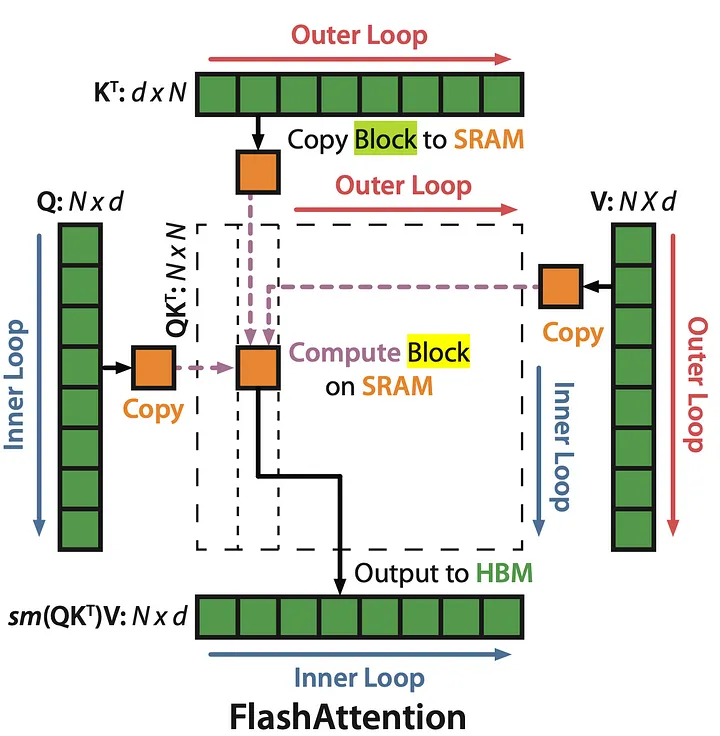
\includegraphics[width=\linewidth]{images/flash_attention_illustration.png}
    \end{column}
  \end{columns}
\end{frame}

\begin{frame}{Softmax: Three Versions}
  \begin{columns}[T]
    \begin{column}{0.48\textwidth}
      \textbf{Naive:} 2 passes. Numerically unstable for large $x_i$.
      \vspace{-0.3em}
      \[
        \text{softmax}(x)_i = \frac{e^{x_i}}{\sum_{j} e^{x_j}}
      \]
      \vspace{-0.8em}

      {\small
      \begin{algorithm}[H]
        \caption{\small Naive Softmax}
        \KwIn{$x = (x_1, \ldots, x_n)$}
        $\ell \gets 0$\;
        \lFor{$i = 1$ \KwTo $n$}{$\ell \gets \ell + e^{x_i}$}
        \lFor{$i = 1$ \KwTo $n$}{$o_i \gets e^{x_i} / \ell$}
        \Return $(o_1, \ldots, o_n)$\;
      \end{algorithm}
      }

      \vspace{0.3em}
      \centering
      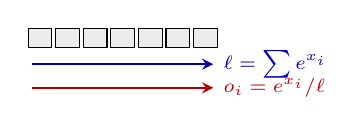
\begin{tikzpicture}[
        cell/.style={draw, fill=gray!15, minimum width=3mm, minimum height=2.5mm, inner sep=0pt},
        arr/.style={-stealth, thick}
      ]
        \foreach \i in {1,...,7} {
          \node[cell] (c\i) at (\i*0.35, 0) {};
        }
        \draw[arr, blue!70!black] ([xshift=-1mm,yshift=-2mm]c1.south) --
          ([xshift=1mm,yshift=-2mm]c7.south) node[right,font=\scriptsize] {$\ell = \sum e^{x_i}$};
        \draw[arr, red!70!black] ([xshift=-1mm,yshift=-5mm]c1.south) --
          ([xshift=1mm,yshift=-5mm]c7.south) node[right,font=\scriptsize] {$o_i = e^{x_i}/\ell$};
      \end{tikzpicture}
    \end{column}
    \begin{column}{0.48\textwidth}
      \textbf{Stable:} 3 passes. Subtract max for numerical stability.
      \vspace{-0.3em}
      \[
        \text{softmax}(x)_i = \frac{e^{x_i - m}}{\sum_{j} e^{x_j - m}}, \; m = \max_j x_j
      \]
      \vspace{-0.8em}

      {\small
      \begin{algorithm}[H]
        \caption{\small Stable Softmax}
        \KwIn{$x = (x_1, \ldots, x_n)$}
        $m \gets -\infty$\;
        \lFor{$i = 1$ \KwTo $n$}{$m \gets \max(m, x_i)$}
        $\ell \gets 0$\;
        \lFor{$i = 1$ \KwTo $n$}{$\ell \gets \ell + e^{x_i - m}$}
        \lFor{$i = 1$ \KwTo $n$}{$o_i \gets e^{x_i - m} / \ell$}
        \Return $(o_1, \ldots, o_n)$\;
      \end{algorithm}
      }

      \vspace{0.3em}
      \centering
      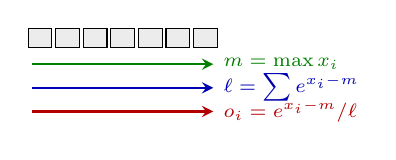
\begin{tikzpicture}[
        cell/.style={draw, fill=gray!15, minimum width=3mm, minimum height=2.5mm, inner sep=0pt},
        arr/.style={-stealth, thick}
      ]
        \foreach \i in {1,...,7} {
          \node[cell] (c\i) at (\i*0.35, 0) {};
        }
        \draw[arr, green!50!black] ([xshift=-1mm,yshift=-2mm]c1.south) --
          ([xshift=1mm,yshift=-2mm]c7.south) node[right,font=\scriptsize] {$m = \max x_i$};
        \draw[arr, blue!70!black] ([xshift=-1mm,yshift=-5mm]c1.south) --
          ([xshift=1mm,yshift=-5mm]c7.south) node[right,font=\scriptsize] {$\ell = \sum e^{x_i - m}$};
        \draw[arr, red!70!black] ([xshift=-1mm,yshift=-8mm]c1.south) --
          ([xshift=1mm,yshift=-8mm]c7.south) node[right,font=\scriptsize] {$o_i = e^{x_i-m}/\ell$};
      \end{tikzpicture}
    \end{column}
  \end{columns}
\end{frame}

\begin{frame}{Streaming (Online) Softmax}
  \begin{columns}[T]
    \begin{column}{0.50\textwidth}
      \begin{itemize}
        \item \textbf{Key insight:} fuse max and sum into a \emph{single pass}
        \item Maintain running max $m$ and rescaled sum $\ell$
        \item When seeing $x_i$:
          \vspace{-0.3em}
          \begin{align*}
            m' &= \max(m, x_i) \\
            \ell' &= \ell \cdot e^{m - m'} + e^{x_i - m'}
          \end{align*}
          \vspace{-0.5em}
        \item The correction $e^{m - m'}$ rescales the previous sum to the new max
      \end{itemize}

      \vspace{0.5em}
      \begin{block}{\small Why this matters}
        {\small 
        \begin{itemize}
        \item Online softmax lets us process $K$ blocks one at a time without knowing the global max
        \item Used in flash attention for streaming output computation
\end{itemize}}
      \end{block}
    \end{column}
    \begin{column}{0.48\textwidth}
      {\small
      \begin{algorithm}[H]
        \caption{\small Online Softmax}
        \KwIn{$x = (x_1, \ldots, x_n)$}
        $m \gets -\infty, \; \ell \gets 0$\;
        \For{$i = 1$ \KwTo $n$}{
          $m' \gets \max(m, x_i)$\;
          $\ell \gets \ell \cdot e^{m - m'} + e^{x_i - m'}$\;
          $m \gets m'$\;
        }
        \lFor{$i = 1$ \KwTo $n$}{$o_i \gets e^{x_i - m} / \ell$}
        \Return $(o_1, \ldots, o_n)$\;
      \end{algorithm}
      }

      \vspace{0.5em}
      \centering
      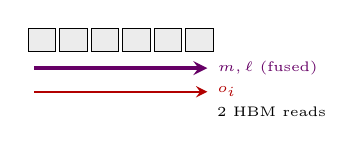
\begin{tikzpicture}[
        cell/.style={draw, fill=gray!15, minimum width=3.5mm, minimum height=3mm, inner sep=0pt},
        arr/.style={-stealth, thick}
      ]
        \foreach \i in {1,...,6} {
          \node[cell] (o\i) at (\i*0.4, 0) {};
        }
        \draw[arr, violet!80!black, line width=1.2pt] ([xshift=-1mm,yshift=-2mm]o1.south) --
          ([xshift=1mm,yshift=-2mm]o6.south) node[right,font=\tiny] {$m, \ell$ (fused)};
        \draw[arr, red!70!black] ([xshift=-1mm,yshift=-5mm]o1.south) --
          ([xshift=1mm,yshift=-5mm]o6.south) node[right,font=\tiny] {$o_i$};
        \node[font=\tiny, anchor=west] at ([xshift=1mm,yshift=-7.5mm]o6.south) {2 HBM reads};
      \end{tikzpicture}
    \end{column}
  \end{columns}
\end{frame}

% -----------------------------------------------------------------------
\subsection{The Flash Attention Algorithm}

\begin{frame}{Attention with Two Blocks}

  \begin{columns}
    \begin{column}{0.58\textwidth}
      Consider a single query block $Q$ attending to keys and values split into two blocks.
      The score matrix and values are partitioned as:
      \[
        S = \begin{bmatrix} S^{(1)} & S^{(2)} \end{bmatrix}, \qquad
        V = \begin{bmatrix} V^{(1)} \\ V^{(2)} \end{bmatrix}
      \]

      To compute softmax over the full row we need the \textbf{global} max and sum:
      \begin{align*}
        m   &= \max\!\big(\text{rowmax}(S^{(1)}),\; \text{rowmax}(S^{(2)})\big) \\
        \ell &= \text{rowsum}(e^{S^{(1)} - m}) + \text{rowsum}(e^{S^{(2)} - m})
      \end{align*}

      The softmax-weighted output becomes:
      \[
        O = \text{diag}(\ell)^{-1}\!\Big(e^{S^{(1)} - m} V^{(1)} + e^{S^{(2)} - m} V^{(2)}\Big)
      \]
    \end{column}
    \begin{column}{0.40\textwidth}
      \centering
      \begin{tikzpicture}[
        blk/.style={draw, thick, inner sep=2pt, font=\scriptsize\bfseries,
                     minimum height=0.7cm},
        arr/.style={-Stealth, thick, gray!70},
        lbl/.style={font=\tiny, text=fagray},
      ]
        \node[blk, fill=orange!25, minimum width=1.3cm] (S1) at (0, 0) {$S^{(1)}$};
        \node[blk, fill=orange!50, minimum width=1.3cm] (S2) at (2.05, 0) {$S^{(2)}$};
        \node[lbl, above=2pt] at ($(S1.north)!0.5!(S2.north)$)
          {$S = QK^\top$};
        \draw[decorate, decoration={brace, mirror, amplitude=3pt}, thick]
          (S1.north west) -- (S1.south west)
          node[midway, left=3pt, font=\tiny] {$B_r$};
        \draw[decorate, decoration={brace, mirror, amplitude=3pt}, thick]
          (S1.south west) -- (S2.south east)
          node[midway, below=3pt, font=\tiny] {$2B_c$};

        \node[lbl, anchor=west] (mlbl) at ($(S2.east) + (0.2, 0.15)$)
          {$\to m$};
        \node[lbl, anchor=west] (llbl) at ($(S2.east) + (0.2,-0.15)$)
          {$\to \ell$};

        \draw[arr] (S1.south) -- ++(0, -0.45)
          node[midway, left, font=\tiny] {$e^{\cdot\, - m}$};
        \draw[arr] (S2.south) -- ++(0, -0.45)
          node[midway, right, font=\tiny] {$e^{\cdot\, - m}$};

        \node[blk, fill=vcol, minimum width=0.9cm, minimum height=0.6cm]
          (V1) at ($(S1.south) + (0, -0.85)$) {$V^{(1)}$};
        \node[blk, fill=vcol!60, minimum width=0.9cm, minimum height=0.6cm]
          (V2) at ($(S2.south) + (0, -0.85)$) {$V^{(2)}$};
        \node[font=\tiny, gray] at ($(V1.east)!0.5!(V2.west)$) {$\times$};
        \node[lbl, right=2pt] at (V2.east) {$B_c \!\times\! d$};

        \node[circle, draw, thick, fill=white, inner sep=1pt,
              font=\scriptsize]
          (plus) at ($(V1.south)!0.5!(V2.south) + (0, -0.6)$) {$+$};
        \draw[arr] (V1.south) -- (plus);
        \draw[arr] (V2.south) -- (plus);

        \node[blk, fill=pink!40, minimum width=0.9cm]
          (O) at ($(plus) + (0, -0.9)$) {$O$};
        \draw[arr] (plus) -- (O)
          node[midway, right, font=\tiny] {$\text{diag}(\ell)^{-1}$};
        \node[lbl, right=2pt] at (O.east) {$B_r \!\times\! d$};
      \end{tikzpicture}

    \end{column}
  \end{columns}

  \vspace{0.3em}
  \begin{alertblock}{Challenge}
    Softmax needs $m$ and $\ell$ across \emph{all} blocks, but we want to process one block at a time.
  \end{alertblock}
\end{frame}

\begin{frame}{Online Softmax for Blocked Attention}
  \begin{columns}[T]
    \begin{column}{0.55\textwidth}
      \textbf{Solution:} Apply streaming softmax to process one block at a time.

      \vspace{0.3em}
      {\small\textbf{After block 1:} local statistics and partial output}
      \vspace{-0.3em}
      \begin{align*}
        m^{(1)} &= \text{rowmax}(S^{(1)}) \\
        \ell^{(1)} &= \text{rowsum}(e^{S^{(1)} - m^{(1)}}) \\
        O^{(1)} &= \text{diag}(\ell^{(1)})^{-1}\, e^{S^{(1)} - m^{(1)}}\, V^{(1)}
      \end{align*}

      \vspace{-0.5em}
      {\small\textbf{After block 2:} update with correction $e^{m^{(1)} - m^{(2)}}$}
      \vspace{-0.3em}
      \begin{align*}
        m^{(2)} &= \max(m^{(1)},\; \text{rowmax}(S^{(2)})) \\
        \ell^{(2)} &= e^{m^{(1)} - m^{(2)}}\, \ell^{(1)} + \text{rowsum}(e^{S^{(2)} - m^{(2)}}) \\
        O^{(2)} &= \tfrac{\ell^{(1)}}{\ell^{(2)}} e^{m^{(1)}-m^{(2)}} O^{(1)}
                 + \tfrac{1}{\ell^{(2)}}\, e^{S^{(2)} - m^{(2)}}\, V^{(2)}
      \end{align*}

      \vspace{-0.3em}
      {\small After the last block: $m^{(2)} \!=\! m$, $\ell^{(2)} \!=\! \ell$, $O^{(2)} \!=\! O$: exact result.}
    \end{column}
    \begin{column}{0.43\textwidth}
      \centering
      \begin{tikzpicture}[
        blk/.style={draw, thick, inner sep=2pt, font=\scriptsize\bfseries,
                     minimum height=0.7cm},
        arr/.style={-Stealth, thick, gray!70},
        lbl/.style={font=\tiny, text=fagray},
      ]
        % === Block 1 (left column) ===
        \node[blk, fill=orange!25, minimum width=1.3cm] (S1) at (0, 0) {$S^{(1)}$};
        \node[lbl, above=2pt] at (S1.north) {$Q K_1^\top$};

        \draw[arr] (S1.south) -- ++(0, -0.4)
          node[midway, left, font=\tiny] {$e^{\cdot\, - m^{(1)}}$};

        \node[blk, fill=vcol, minimum width=0.9cm, minimum height=0.6cm]
          (V1) at ($(S1.south) + (0, -0.8)$) {$V^{(1)}$};

        % Stats after block 1
        \node[draw, thick, rounded corners=2pt, fill=blue!10,
              inner sep=2pt, font=\tiny, minimum width=1.1cm]
          (st1) at ($(V1.south) + (0, -0.65)$) {$m^{(1)}, \ell^{(1)}$};
        \draw[arr] (V1.south) -- (st1.north);

        \node[blk, fill=pink!25, minimum width=0.9cm]
          (O1) at ($(st1.south) + (0, -0.8)$) {$O^{(1)}$};
        \draw[arr] (st1.south) -- (O1.north);

        % === Block 2 (right column) ===
        \node[blk, fill=orange!50, minimum width=1.3cm] (S2) at (2.8, 0) {$S^{(2)}$};
        \node[lbl, above=2pt] at (S2.north) {$Q K_2^\top$};

        \draw[arr] (S2.south) -- ++(0, -0.4)
          node[midway, right, font=\tiny] {$e^{\cdot\, - m^{(2)}}$};

        \node[blk, fill=vcol!60, minimum width=0.9cm, minimum height=0.6cm]
          (V2) at ($(S2.south) + (0, -0.8)$) {$V^{(2)}$};

        % Streaming softmax update: stats from block 1 feed into block 2
        \node[draw, thick, rounded corners=2pt, fill=blue!20,
              inner sep=2pt, font=\tiny, minimum width=1.1cm]
          (st2) at ($(V2.south) + (0, -0.65)$) {$m^{(2)}, \ell^{(2)}$};
        \draw[arr] (V2.south) -- (st2.north);

        % Rescale arrow from block 1 stats to block 2 stats
        \draw[arr, violet!80!black, line width=1pt]
          (st1.east) -- (st2.west)
          node[midway, above, font=\tiny, violet!80!black] {$\cdot\, e^{m^{(1)} - m^{(2)}}$};

        % Plus node below st2
        \node[circle, draw, thick, fill=white, inner sep=1pt,
              font=\scriptsize]
          (plus) at ($(st2.south) + (0, -0.7)$) {$+$};

        % Rescale O^(1) into plus
        \coordinate (elbow) at (O1.east |- plus.west);
        \draw[arr, violet!80!black, line width=1pt] (O1.east) -- (elbow) -- (plus.west);
        \node[above, font=\tiny, violet!80!black] at ($(elbow)!0.5!(plus.west)$) {rescale};

        % New contribution from block 2 into plus
        \draw[arr] (st2.south) -- (plus.north)
          node[midway, right, font=\tiny] {$\tilde{P}^{(2)} V^{(2)}$};

        % Final O below plus
        \node[blk, fill=pink!40, minimum width=0.9cm]
          (O) at ($(plus) + (0, -0.9)$) {$O$};
        \draw[arr] (plus) -- (O)
          node[midway, right, font=\tiny] {$\text{diag}(\ell^{(2)})^{-1}$};
        \node[lbl, right=2pt] at (O.east) {$B_r \!\times\! d$};
      \end{tikzpicture}
    \end{column}
  \end{columns}
\end{frame}

\begin{frame}{Flash Attention 2: Forward Pass}

  \begin{columns}[T]
    \begin{column}{0.55\textwidth}
      {\small
      \begin{algorithm}[H]
        \caption{\small FlashAttention-2 Forward}
        \KwIn{$Q, K, V \in \mathbb{R}^{T \times d}$ in HBM; block sizes $B_r, B_c$}
        \KwOut{$O \in \mathbb{R}^{T \times d}$, $L \in \mathbb{R}^{T}$}
        Split $Q$ into $T_r$ row-blocks $Q_i \!\in\! \mathbb{R}^{B_r \times d}$; $K, V$ into $T_c$ row-blocks $K_j, V_j \!\in\! \mathbb{R}^{B_c \times d}$. Output $O$ likewise has row-blocks $O_i \!\in\! \mathbb{R}^{B_r \times d}$\;
        \For{$i = 1, \ldots, T_r$}{
          \textcolor{loadcol}{Load $Q_i$ from HBM to SRAM}\;
          $O_i \gets 0$, $\ell_i \gets 0$, $m_i \gets -\infty$\;
          \For{$j = 1, \ldots, T_c$}{
            \textcolor{loadcol}{Load $K_j, V_j$ from HBM to SRAM}\;
            \textcolor{compcol}{$S_{ij} \gets Q_i K_j^\top$}\;
            \textcolor{compcol}{$\tilde{m}_i \gets \max(m_i, \operatorname{rowmax}(S_{ij}))$}\;
            \textcolor{compcol}{$\tilde{P}_{ij} \gets \exp(S_{ij} - \tilde{m}_i)$}\;
            \textcolor{compcol}{$\ell_i \gets e^{m_i - \tilde{m}_i} \ell_i + \operatorname{rowsum}(\tilde{P}_{ij})$}\;
            \textcolor{compcol}{$O_i \gets \operatorname{diag}(e^{m_i - \tilde{m}_i}) O_i + \tilde{P}_{ij} V_j$}\;
            $m_i \gets \tilde{m}_i$\;
          }
          \textcolor{compcol}{$O_i \gets \operatorname{diag}(\ell_i)^{-1} O_i$} \tcp*{Trick 1}
          $L_i \gets m_i + \log(\ell_i)$ \tcp*{Trick 2}
          \textcolor{storecol}{Write $O_i$, $L_i$ to HBM}\;
        }
        \Return $O$, $L$\;
      \end{algorithm}
      }

      \vspace{0.3em}
      {\small
      \begin{description}
        \item[Trick 1:] Accumulate unnormalized $O_i$, divide by $\ell_i$ once at the end.
        \item[Trick 2:] Store $L_i = m_i + \log(\ell_i)$ instead of $m_i$ and $\ell_i$ separately (for backward pass).
      \end{description}
      }
    \end{column}
    \begin{column}{0.43\textwidth}
      \centering
      \resizebox{\linewidth}{!}{%
      \begin{tikzpicture}[
        font=\sffamily\scriptsize,
        qblk/.style={draw, thick, minimum width=13mm, minimum height=5.5mm, inner sep=0pt, fill=blue!12, text height=1.4ex, text depth=.4ex, anchor=center},
        qcur/.style={draw, very thick, minimum width=13mm, minimum height=5.5mm, inner sep=0pt, fill=blue!55, text=white, font=\scriptsize\bfseries, text height=1.4ex, text depth=.4ex, anchor=center},
        kblk/.style={draw, thick, minimum width=22mm, minimum height=5.5mm, inner sep=0pt, fill=fagreen!25, text height=1.4ex, text depth=.4ex, anchor=center},
        kcur/.style={draw, very thick, minimum width=22mm, minimum height=5.5mm, inner sep=0pt, fill=fagreen!60, text=white, font=\scriptsize\bfseries, text height=1.4ex, text depth=.4ex, anchor=center},
        oblk/.style={draw, thick, minimum width=13mm, minimum height=5.5mm, inner sep=0pt, fill=pink!25, text height=1.4ex, text depth=.4ex, anchor=center},
        ocur/.style={draw, very thick, minimum width=13mm, minimum height=5.5mm, inner sep=0pt, fill=pink!70, font=\scriptsize\bfseries, text height=1.4ex, text depth=.4ex, anchor=center},
        arr/.style={-Stealth, line width=1pt},
      ]
        \def\dy{0.55}
        \def\xQ{0}
        \def\xK{2.45}
        \def\xO{5.0}

        % Column headers
        \node[font=\bfseries] at (\xQ, 0.6) {$Q$};
        \node[font=\bfseries] at (\xK, 0.6) {$K,\ V$};
        \node[font=\bfseries] at (\xO, 0.6) {$O$};

        % Q column (touching row-blocks, evenly spaced)
        \node[qblk] (Q1) at (\xQ, 0) {$Q_1$};
        \node[qblk] (Q2) at (\xQ, -\dy) {$Q_2$};
        \node[qcur] (Qi) at (\xQ, -2*\dy) {$Q_i$};
        \node[qblk] (Q4) at (\xQ, -3*\dy) {$Q_{T_r-1}$};
        \node[qblk] (Q5) at (\xQ, -4*\dy) {$Q_{T_r}$};

        % K, V column (each block represents the K_j, V_j pair)
        \node[kblk] (K1) at (\xK, 0) {$K_1,\, V_1$};
        \node[kblk] (K2) at (\xK, -\dy) {$K_2,\, V_2$};
        \node[kcur] (Kj) at (\xK, -2*\dy) {$K_j,\, V_j$};
        \node[kblk] (K4) at (\xK, -3*\dy) {$K_{T_c-1},\, V_{T_c-1}$};
        \node[kblk] (K5) at (\xK, -4*\dy) {$K_{T_c},\, V_{T_c}$};

        % O column
        \node[oblk] (O1) at (\xO, 0) {$O_1$};
        \node[oblk] (O2) at (\xO, -\dy) {$O_2$};
        \node[ocur] (Oi) at (\xO, -2*\dy) {$O_i$};
        \node[oblk] (O4) at (\xO, -3*\dy) {$O_{T_r-1}$};
        \node[oblk] (O5) at (\xO, -4*\dy) {$O_{T_r}$};

        % Outer-loop arrow, well to the left of Q (no overlap)
        \draw[arr, blue!70!black] ([xshift=-8mm] Q1.west) -- ([xshift=-8mm] Q5.west);
        \node[blue!70!black, font=\scriptsize\bfseries, rotate=90]
          at ([xshift=-12mm] $(Q1)!0.5!(Q5)$) {outer $i$};

        % Inner-loop arrow in the gap between K,V column and O column
        \draw[arr, fagreen!70!black] ([xshift=5mm] K1.east) -- ([xshift=5mm] K5.east);
        \node[fagreen!70!black, font=\scriptsize\bfseries, rotate=-90]
          at ([xshift=9mm] $(K1)!0.5!(K5)$) {inner $j$};

        % Bottom captions
        \node[anchor=north, align=center, font=\scriptsize] at ($(Q5)+(0,-0.5)$)
          {$Q_i \!\in\! \mathbb{R}^{B_r\times d}$\\loaded once per $i$};
        \node[anchor=north, align=center, font=\scriptsize] at ($(K5)+(0,-0.5)$)
          {$K_j, V_j \!\in\! \mathbb{R}^{B_c\times d}$\\streamed across $j$};
        \node[anchor=north, align=center, font=\scriptsize] at ($(O5)+(0,-0.5)$)
          {$O_i \!\in\! \mathbb{R}^{B_r\times d}$\\written once per $i$};
      \end{tikzpicture}}

      \vspace{0.4em}
      {\scriptsize
      For each outer $i$: load $Q_i$, loop over all $K_j, V_j$ in SRAM, write back $O_i$. No $T\!\times\!T$ matrix ever materialized.
      }
    \end{column}
  \end{columns}
\end{frame}

\begin{frame}{Attention Backward Pass: Gradient Derivation}
  \textbf{Forward:} $S = QK^\top$, \; $P = \text{softmax}(S)$, \; $O = PV$. \;
  Given $dO$, derive $dQ, dK, dV$.

  \vspace{0.6em}
  \begin{description}
    \item[Through $O = PV$:] \quad $dV = P^\top dO$, \quad $dP = dO\, V^\top$
    \item[Through softmax (row-wise):] Jacobian $\partial P_i/\partial S_i = \text{diag}(P_i) - P_i P_i^\top$, so
      \vspace{-0.3em}
      \[
        dS_i = P_i \odot dP_i - D_i\, P_i,
        \qquad D_i := P_i^\top dP_i = \sum_j P_{ij}\, dP_{ij}
      \]
      \vspace{-1.0em}
      \begin{center}
        Componentwise: $\; dS_{ij} = P_{ij}(dP_{ij} - D_i)$
      \end{center}
    \item[Through $S = QK^\top$:] \quad $dQ = dS \cdot K$, \quad $dK = dS^\top \cdot Q$
  \end{description}

  \vspace{0.6em}
  \begin{alertblock}{What we still need block-wise}
    Computing $dV, dS, dQ, dK$ requires $P$ and $dP$. Naively that means writing the $T \times T$ matrices to HBM. Next two slides: how to avoid that.
  \end{alertblock}
\end{frame}

\begin{frame}{Avoiding $P$ and $dP$ in HBM}

  \textbf{Observation.} Substitute $dP_{ij} = \sum_k dO_{ik} V_{jk}$ into $D_i$:
  \vspace{-0.3em}
  \[
    D_i = \sum_j P_{ij} \sum_k dO_{ik} V_{jk}
        = \sum_k dO_{ik} \underbrace{\sum_j P_{ij} V_{jk}}_{= O_{ik}}
        = \sum_k dO_{ik}\, O_{ik}
  \]
  \vspace{-0.3em}
  \[
    \boxed{\; D = \text{rowsum}(dO \odot O) \;}
  \]

  \vspace{0.4em}
  \textbf{Why this matters.} $D$ depends only on $dO$ and $O$, not on $P$ or $dP$.

  \vspace{0.4em}
  \textbf{Backward streaming pattern:}
  \begin{enumerate}
    \item Precompute $D \in \mathbb{R}^{T}$ from $dO, O$ in one pass
    \item For each $(i,j)$ block: recompute $S_{ij}, P_{ij}, dP_{ij}$ in SRAM, then accumulate into $dQ, dK, dV$
  \end{enumerate}

  \vspace{0.4em}
  \begin{alertblock}{Result}
    Neither $P$ nor $dP$ is ever materialized in HBM as a $T \times T$ matrix.
  \end{alertblock}
\end{frame}

\begin{frame}{Recomputing $P$ from the Stored Log-Sum-Exp $L$}

  The forward stored \emph{one scalar per row}, $L_i = m_i + \log \ell_i$, with $m_i = \max_j S_{ij}$ and $\ell_i = \sum_j e^{S_{ij} - m_i}$.

  \vspace{0.4em}
  \textbf{Backward identity:}
  \vspace{-0.3em}
  \[
    P_{ij} = \frac{e^{S_{ij} - m_i}}{\ell_i}
           = e^{S_{ij} - m_i - \log \ell_i}
           = e^{S_{ij} - L_i}
  \]

  \vspace{-0.2em}
  Recipe: recompute $S_{ij} = Q_i K_j^\top$ block-wise in SRAM, then $P_{ij} = \exp(S_{ij} - L_i)$.

  \vspace{0.5em}
  \begin{description}
    \item[One scalar per row.] $L_i$ replaces $(m_i, \ell_i)$, fuses normalization into a single $\exp$
    \item[Numerically stable.] $L_i \geq m_i \geq S_{ij} \Rightarrow \exp(S_{ij} - L_i) \in (0, 1]$
    \item[Memory vs.\ compute.] One extra $QK^\top$ block-matmul, no $T \times T$ matrix in HBM
    \item[Sole forward-to-backward link.] $L$ is the only auxiliary (besides $O$) carried over, justifying ``$L_i \gets m_i + \log \ell_i$'' (\emph{Trick 2}) in the forward
  \end{description}
\end{frame}

\begin{frame}{Flash Attention 2: Backward Pass}
  \begin{columns}[T]
    \begin{column}{0.55\textwidth}
      {\small
      \begin{algorithm}[H]
        \caption{\small FlashAttention-2 Backward}
        \KwIn{$Q, K, V, O, dO \in \mathbb{R}^{T \times d}$, $L \in \mathbb{R}^{T}$ in HBM; block sizes $B_r, B_c$}
        \KwOut{$dQ, dK, dV \in \mathbb{R}^{T \times d}$}
        Divide $K, V$ into $T_c$ blocks; $Q, O, dO, dQ$ into $T_r$ blocks\;
        $D \gets \operatorname{rowsum}(dO \odot O)$ \tcp*{precompute}
        \For{$j = 1, \ldots, T_c$}{
          \textcolor{loadcol}{Load $K_j, V_j$ from HBM}\;
          $dK_j \gets 0$, $dV_j \gets 0$\;
          \For{$i = 1, \ldots, T_r$}{
            \textcolor{loadcol}{Load $Q_i, O_i, dO_i, L_i, D_i$}\;
            \textcolor{compcol}{$S_{ij} \gets Q_i K_j^\top$}\;
            \textcolor{compcol}{$P_{ij} \gets \exp(S_{ij} - L_i)$} \tcp*{recompute}
            \textcolor{compcol}{$dV_j \gets dV_j + P_{ij}^\top\, dO_i$}\;
            \textcolor{compcol}{$dP_{ij} \gets dO_i\, V_j^\top$}\;
            \textcolor{compcol}{$dS_{ij} \gets P_{ij} \odot (dP_{ij} - D_i)$}\;
            \textcolor{compcol}{$dQ_i \gets dQ_i + dS_{ij}\, K_j$}\;
            \textcolor{compcol}{$dK_j \gets dK_j + dS_{ij}^\top\, Q_i$}\;
          }
          \textcolor{storecol}{Write $dK_j$, $dV_j$ to HBM}\;
        }
        \Return $dQ, dK, dV$\;
      \end{algorithm}
      }
    \end{column}
    \begin{column}{0.43\textwidth}
      \centering
      \begin{tikzpicture}[
        mat/.style={draw, thick, minimum width=5mm, minimum height=5mm,
                    inner sep=0pt, font=\tiny\bfseries,
                    text depth=.5ex, text height=1.5ex},
        sram/.style={draw, thick, rounded corners=3pt, dashed,
                     fill=fasram!15, inner sep=4pt},
        hbm/.style={draw, thick, rounded corners=3pt,
                    fill=fahbm!15, inner sep=4pt},
        arr/.style={-Stealth, thick, gray!60},
        lbl/.style={font=\tiny},
      ]
        % HBM region
        \node[hbm, minimum width=3.4cm, minimum height=1.2cm] (hbmbox) at (0, 2.8) {};
        \node[lbl, anchor=north west] at (hbmbox.north west) {HBM};

        % K, V in HBM (left side)
        \foreach \i/\c in {1/green!20, 2/green!35, 3/green!50, 4/green!65} {
          \node[mat, fill=\c, minimum width=3.5mm] (K\i) at (-1.6+\i*0.35, 2.65) {};
        }
        \node[lbl, above=1pt] at ($(K2.north)!0.5!(K3.north)$) {$K,V$};

        % Q, dO, O, L in HBM (shifted left, closer to K)
        \foreach \i/\c in {1/blue!20, 2/blue!35, 3/blue!50} {
          \node[mat, fill=\c, minimum width=3.5mm] (Q\i) at (0.2+\i*0.35, 2.65) {};
        }
        \node[lbl, above=1pt] at (Q2.north) {$Q,dO,O,L$};

        % SRAM region (shorter and wider, mirrors HBM layout)
        \node[sram, minimum width=3.6cm, minimum height=1.6cm] (srambox) at (0.1, 0.5) {};
        \node[lbl, anchor=north west] at (srambox.north west) {SRAM};

        % K_j, V_j in SRAM (stays)
        \node[mat, fill=green!40, minimum width=8mm, minimum height=6mm]
          (KVj) at (-1.05, 0.45) {$\mathstrut K_j\!,V_j$};
        \node[lbl, anchor=base] at (-1.05, -0.05) {stays};

        % Q_i, dO_i block (streamed)
        \node[mat, fill=blue!35, minimum width=8mm, minimum height=6mm]
          (Qi) at (0.1, 0.45) {$\mathstrut Q_i\!,dO_i$};
        \node[lbl, anchor=base] at (0.1, -0.05) {streamed};

        % dK_j, dV_j accumulators
        \node[mat, fill=red!20, minimum width=8mm, minimum height=6mm]
          (dKV) at (1.25, 0.45) {$\mathstrut dK_j\!,dV_j$};
        \node[lbl, anchor=base] at (1.25, -0.05) {accum.};

        % Arrows
        \draw[arr, loadcol] (K2.south) -- (KVj.north)
          node[midway, left, lbl] {once};
        \draw[arr, loadcol] (Q2.south) -- (Qi.north)
          node[midway, right, lbl] {loop};
        \draw[arr, storecol] (dKV.north) -- (dKV.north |- hbmbox.south)
          node[midway, right, lbl] {once};

        % Legend
        \node[lbl, loadcol, anchor=west] at (-1.5, -0.7) {$\blacksquare$ Load};
        \node[lbl, compcol, anchor=west] at (-0.4, -0.7) {$\blacksquare$ Compute};
        \node[lbl, storecol, anchor=west] at (0.7, -0.7) {$\blacksquare$ Store};
      \end{tikzpicture}

      \vspace{0.3em}
      {\small
      \textbf{Key differences from forward:}
      \begin{itemize}
        \item Outer loop over $K, V$ blocks (not $Q$)
        \item $P_{ij}$ recomputed from $Q_i, K_j, L_i$
        \item $D_i$ avoids storing $P$
      \end{itemize}
      }
    \end{column}
  \end{columns}
\end{frame}

% -----------------------------------------------------------------------
\subsection{GPU Programming: CUDA and Triton}

\begin{frame}{CUDA Programming Model}

  \begin{columns}[T]
    \begin{column}{0.40\textwidth}
      \textbf{CUDA} is NVIDIA's programming model for GPUs.

      \vspace{0.3em}
      \begin{itemize}\small
        \item \textbf{Thread}: runs the kernel
        \item \textbf{Warp}: 32 threads executing in lockstep (SIMT); implicit, not exposed in CUDA code
        \item \textbf{Block}: up to 1024 threads, runs on one SM
        \item \textbf{Grid}: collection of blocks, launched on the GPU
      \end{itemize}

      \vspace{0.4em}
      \centering
      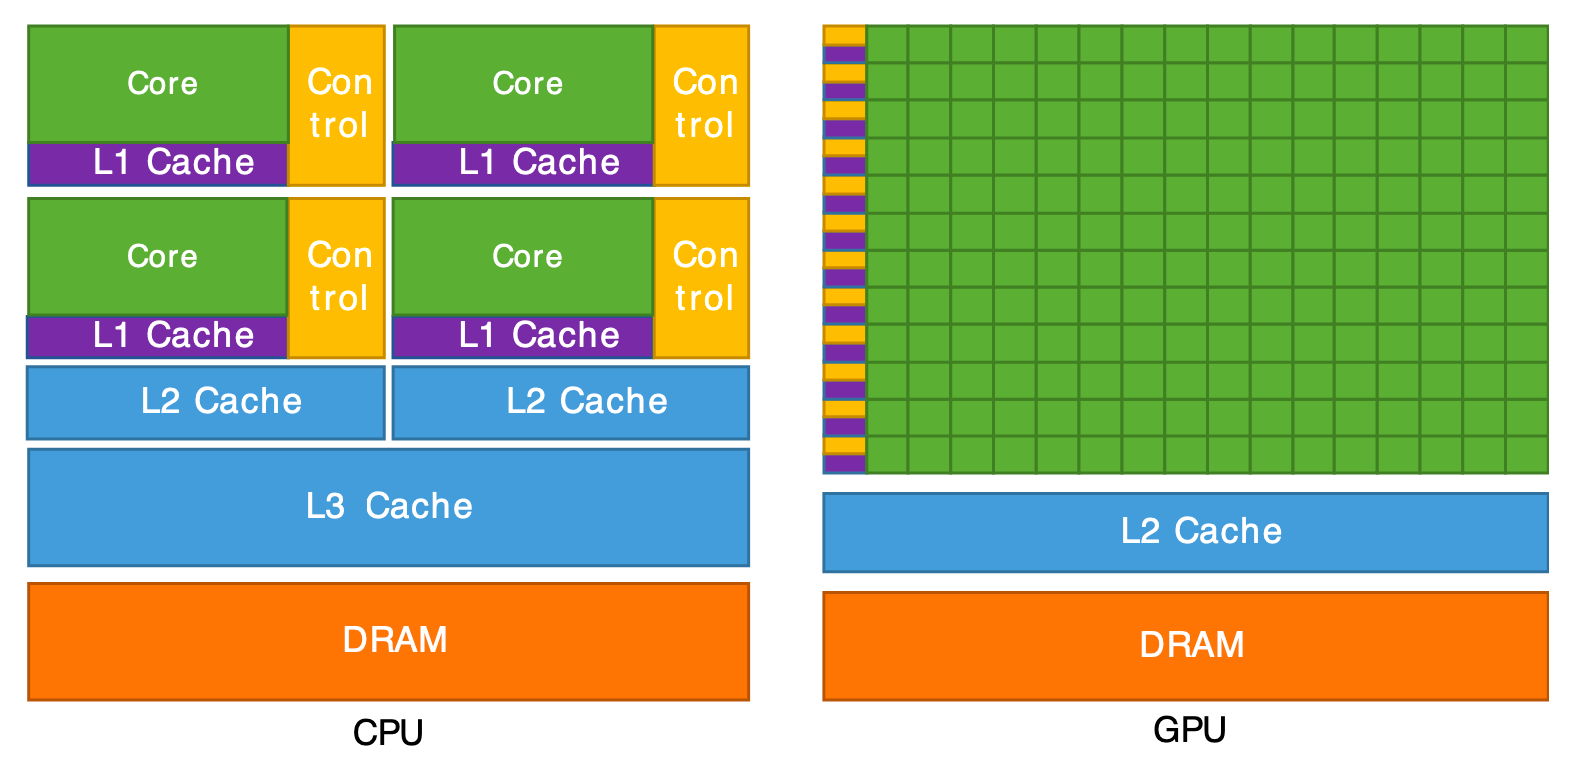
\includegraphics[width=0.95\linewidth]{images/CPU_vs_GPU2.png}
    \end{column}
    \begin{column}{0.58\textwidth}
      \centering
      \begin{tikzpicture}[
        >=Stealth,
        every node/.style={font=\scriptsize},
        scale=0.85, transform shape,
      ]
        % --- Grid ---
        \node[font=\small\bfseries, anchor=south] at (3.1, 4.05) {Grid (launched on GPU)};
        \draw[thick, fablue, fill=fablue!8, rounded corners=2pt] (0, 1.6) rectangle (6.2, 4.0);
        \foreach \x in {0,1,2,3} {
          \foreach \y in {0,1} {
            \pgfmathsetmacro{\xx}{0.4 + \x*1.4}
            \pgfmathsetmacro{\yy}{1.85 + \y*0.95}
            \draw[fill=fablue!35, thick, draw=fablue!80, rounded corners=1pt]
              (\xx, \yy) rectangle (\xx+1.2, \yy+0.78);
            \node[font=\scriptsize] at (\xx+0.6, \yy+0.39) {block};
          }
        }
        % highlighted block (the one we zoom into)
        \draw[ultra thick, fared, rounded corners=1pt] (1.8, 1.85) rectangle (3.0, 2.63);

        % --- Zoom-in (explosion) lines ---
        \draw[dashed, fared, semithick] (1.8, 1.85) -- (0, 0.5);
        \draw[dashed, fared, semithick] (3.0, 1.85) -- (6.2, 0.5);

        % --- Block ---
        \node[font=\small\bfseries, anchor=south] at (3.1, 0.5) {Block (executed on one SM)};
        \draw[thick, fared, fill=fared!5, rounded corners=2pt] (0, -2.5) rectangle (6.2, 0.5);

        % Warps as colored rows of 32 thread cells
        \foreach \w/\warpcolor in {0/fagreen, 1/fablue, 2/fasram, 3/fagray} {
          \pgfmathsetmacro{\ypos}{0.2 - \w*0.6}
          \node[font=\tiny, anchor=east] at (1.05, \ypos-0.22) {warp \w};
          \foreach \i in {0,...,31} {
            \pgfmathsetmacro{\xpos}{1.1 + \i*0.155}
            \draw[fill=\warpcolor!50, draw=\warpcolor!90, line width=0.15pt]
              (\xpos, \ypos) rectangle (\xpos+0.145, \ypos-0.45);
          }
        }
        % brace under one full warp row (warp 3)
        \draw[decorate, decoration={brace, amplitude=3pt, mirror}, fagray, thick]
          (1.1, -2.05) -- (6.06, -2.05);
        \node[font=\tiny, anchor=north] at (3.58, -2.12) {32 threads = 1 warp (lockstep, SIMT)};
      \end{tikzpicture}
    \end{column}
  \end{columns}
\end{frame}

\begin{frame}[fragile]{CUDA Example: Vector Addition}

\begin{lstlisting}[language=C++, keywordstyle=\color{fablue}\bfseries]
__global__ void cuda_vector_add(float *OUT, float *A, float *B, int N)
{
    int i = threadIdx.x;
    if (i < N) { OUT[i] = A[i] + B[i]; }
}

// Allocate device memory and copy host vectors to GPU
float *d_A, *d_B, *d_OUT;
cudaMalloc(&d_A,   N * sizeof(float));
cudaMalloc(&d_B,   N * sizeof(float));
cudaMalloc(&d_OUT, N * sizeof(float));
cudaMemcpy(d_A, h_A, N * sizeof(float), cudaMemcpyHostToDevice);
cudaMemcpy(d_B, h_B, N * sizeof(float), cudaMemcpyHostToDevice);

// Launch: one block, N threads
cuda_vector_add<<<1, N>>>(d_OUT, d_A, d_B, N);
\end{lstlisting}

  \vspace{0.2em}
  {\scriptsize
  \begin{itemize}
    \item \texttt{\_\_global\_\_}: marks a function as a \emph{kernel}: callable from the host, runs on the device.
    \item \texttt{cudaMalloc} / \texttt{cudaMemcpy}: allocate GPU memory and transfer data from host to device.
    \item \texttt{threadIdx.x}: built-in index of the current thread within its block (here the only block).
    \item \texttt{<{}<{}<1, N>{}>{}>}: launch configuration: 1 block of $N$ threads. Each thread computes one element \texttt{OUT[i] = A[i] + B[i]}.
  \end{itemize}
  }
\end{frame}

\begin{frame}[fragile]{CUDA Example: Matrix Addition}

\begin{lstlisting}[language=C++, keywordstyle=\color{fablue}\bfseries]
__global__ void cuda_matrix_add(float *OUT, float *A, float *B,
                                 int NUM_ROWS, int NUM_COLS)
{
    int row = blockIdx.y * blockDim.y + threadIdx.y;
    int col = blockIdx.x * blockDim.x + threadIdx.x;
    if (row < NUM_ROWS && col < NUM_COLS) {
        size_t idx = row * NUM_COLS + col;
        OUT[idx] = A[idx] + B[idx];
    }
}

// 2D grid and block layout
dim3 grid(ceil(NUM_COLS/16), ceil(NUM_ROWS/16), 1);
dim3 block(16, 16, 1);
cuda_matrix_add<<<grid, block>>>(d_OUT, d_A, d_B, NUM_ROWS, NUM_COLS);
\end{lstlisting}

  \vspace{0.3em}
  {\scriptsize
  \begin{itemize}
    \item \texttt{block(16, 16, 1)}: each block contains $16 \times 16 = 256$ threads, arranged as a 2D tile that covers a $16 \times 16$ patch of the matrix.
    \item \texttt{grid(ceil(NUM\_COLS/16), ceil(NUM\_ROWS/16), 1)}: enough blocks to tile the entire matrix; \texttt{ceil} rounds up so partial tiles at the boundary are still covered (the \texttt{if} guards out-of-range threads).
    \item 2D indexing: \texttt{blockIdx} selects the tile, \texttt{threadIdx} selects the element within the tile.
  \end{itemize}
  }

  \vspace{0.3em}
  {\scriptsize
  \begin{block}{Why not a single block as in vector addition?}
    \begin{itemize}
      \item A block is capped at $1024$ threads: \texttt{<{}<{}<1, N>{}>{}>} only works for tiny inputs.
      \item One block runs on a single SM; many blocks run in parallel across all SMs.
    \end{itemize}
  \end{block}
  }
\end{frame}

\begin{frame}{Tensor Memory Layout}

  Tensors are flat arrays in memory, described by \textbf{shape} and \textbf{strides}:
  \begin{itemize}\small
    \item \textbf{shape}: number of elements per dimension
    \item \textbf{stride}: number of elements to skip in memory to advance one step in that dimension
  \end{itemize}

  \vspace{0.4em}
  \centering
  % --- Vector layout ---
  \begin{tikzpicture}[
    font=\scriptsize,
    cell/.style={draw=fagray!70, minimum width=6mm, minimum height=6mm, inner sep=0pt, font=\scriptsize},
  ]
    \node[anchor=east, font=\small] at (-0.15, 0.8) {logical:};
    \foreach \i/\v in {0/1, 1/2, 2/3, 3/5, 4/8, 5/13, 6/21} {
      \node[cell, fill=fablue!15] (l\i) at (\i*0.7, 0.8) {$\v$};
    }
    \foreach \i in {0,...,6} {
      \node[font=\tiny, fagray, above=-1pt of l\i] {[\i]};
    }
    \node[anchor=east, font=\small] at (-0.15, -0.8) {memory:};
    \foreach \i/\v in {0/1, 1/2, 2/3, 3/5, 4/8, 5/13, 6/21} {
      \node[cell, fill=fagreen!15] (p\i) at (\i*0.7, -0.8) {$\v$};
    }
    \foreach \i/\addr in {0/100, 1/104, 2/108, 3/112, 4/116, 5/120, 6/124} {
      \node[font=\tiny, fagray, below=-1pt of p\i] {\addr};
    }
    \node[anchor=west, font=\small] at (5.4, 0.4) {1D vector:\; shape $= [7]$};
    \node[anchor=west, font=\small] at (5.4, -0.4) {\hphantom{1D vector:\;} stride $= [1]$};
  \end{tikzpicture}

  \vspace{0.5em}
  % --- Matrix layout (row-major) ---
  \begin{tikzpicture}[
    font=\scriptsize,
    cell/.style={draw=fagray!70, minimum width=6mm, minimum height=6mm, inner sep=0pt, font=\scriptsize},
  ]
    \node[anchor=south, font=\small] at (0.7, 1.55) {logical $(2{\times}3)$};
    \foreach \j/\v in {0/1, 1/2, 2/3} {
      \node[cell, fill=fablue!25] (m0\j) at (\j*0.7, 0.85) {$\v$};
    }
    \foreach \j/\v in {0/5, 1/8, 2/13} {
      \node[cell, fill=fasram!35] (m1\j) at (\j*0.7, 0.15) {$\v$};
    }
    \node[font=\tiny, fagray, left=2pt of m00] {row 0};
    \node[font=\tiny, fagray, left=2pt of m10] {row 1};

    \node[anchor=south, font=\small] at (5.5, 1.55) {memory (row-major)};
    \foreach \i/\v/\c in {0/1/fablue!25, 1/2/fablue!25, 2/3/fablue!25, 3/5/fasram!35, 4/8/fasram!35, 5/13/fasram!35} {
      \node[cell, fill=\c] (p\i) at (3.4 + \i*0.7, 0.5) {$\v$};
    }
    \foreach \i/\addr in {0/62, 1/66, 2/70, 3/74, 4/78, 5/82} {
      \node[font=\tiny, fagray, below=-1pt of p\i] {\addr};
    }
    \draw[decorate, decoration={brace, amplitude=2pt}, fagray]
      (p0.north west) -- node[above=2pt, font=\tiny] {row 0} (p2.north east);
    \draw[decorate, decoration={brace, amplitude=2pt}, fagray]
      (p3.north west) -- node[above=2pt, font=\tiny] {row 1} (p5.north east);

    \node[anchor=west, font=\small] at (8.0, 0.85) {2D matrix:\; shape $= [2,3]$};
    \node[anchor=west, font=\small] at (8.0, 0.30) {\hphantom{2D matrix:\;} stride $= [3,1]$};
    \node[anchor=west, font=\tiny, fagray, align=left] at (8.0, -0.30)
      {next row $\to +3$, next col $\to +1$};
  \end{tikzpicture}
\end{frame}

\begin{frame}[fragile]{Naive Matrix Multiplication in CUDA}
\begin{columns}[T]
  \begin{column}{0.55\textwidth}
\begin{lstlisting}[language=C++, keywordstyle=\color{fablue}\bfseries, basicstyle=\ttfamily\scriptsize]
// C = A * B, with A: M x K, B: K x N, C: M x N
__global__ void cuda_matmul_naive(float *C, float *A, float *B,
                                  int M, int N, int K)
{
    int row = blockIdx.y * blockDim.y + threadIdx.y;
    int col = blockIdx.x * blockDim.x + threadIdx.x;
    if (row < M && col < N) {
        float sum = 0.0f;
        for (int k = 0; k < K; ++k)
            sum += A[row * K + k] * B[k * N + col];
        C[row * N + col] = sum;
    }
}

dim3 grid(ceil(N/16.0), ceil(M/16.0), 1);
dim3 block(16, 16, 1);
cuda_matmul_naive<<<grid, block>>>(d_C, d_A, d_B, M, N, K);
\end{lstlisting}
  \end{column}
  \begin{column}{0.45\textwidth}
    \centering
    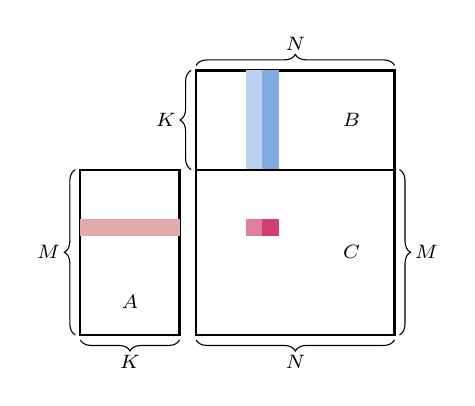
\begin{tikzpicture}[scale=0.42, font=\tiny]
      % --- B (top): K rows x N cols ---
      \draw[thick] (3.5, 5) rectangle (9.5, 8);
      \fill[fablue!30] (5.0, 5) rectangle (5.5, 8);
      \fill[fablue!55] (5.5, 5) rectangle (6.0, 8);
      \node[font=\scriptsize] at (8.2, 6.5) {$B$};
      \draw[decorate, decoration={brace, amplitude=4pt}]
        (3.5, 8.15) -- (9.5, 8.15)
        node[midway, above=2pt, font=\scriptsize] {$N$};
      \draw[decorate, decoration={brace, amplitude=4pt}]
        (3.35, 5) -- (3.35, 8)
        node[midway, left=2pt, font=\scriptsize] {$K$};

      % --- A (left): M rows x K cols ---
      \draw[thick] (0, 0) rectangle (3, 5);
      \fill[fared!40] (0, 3.0) rectangle (3, 3.5);
      \node[font=\scriptsize] at (1.5, 1.0) {$A$};
      \draw[decorate, decoration={brace, amplitude=4pt}]
        (-0.15, 0) -- (-0.15, 5)
        node[midway, left=2pt, font=\scriptsize] {$M$};
      \draw[decorate, decoration={brace, amplitude=4pt, mirror}]
        (0, -0.15) -- (3, -0.15)
        node[midway, below=2pt, font=\scriptsize] {$K$};

      % --- C (bottom right): M rows x N cols ---
      \draw[thick] (3.5, 0) rectangle (9.5, 5);
      \fill[purple!50] (5.0, 3.0) rectangle (5.5, 3.5);
      \fill[purple!75] (5.5, 3.0) rectangle (6.0, 3.5);
      \node[font=\scriptsize] at (8.2, 2.5) {$C$};
      \draw[decorate, decoration={brace, amplitude=4pt}]
        (9.65, 5) -- (9.65, 0)
        node[midway, right=2pt, font=\scriptsize] {$M$};
      \draw[decorate, decoration={brace, amplitude=4pt, mirror}]
        (3.5, -0.15) -- (9.5, -0.15)
        node[midway, below=2pt, font=\scriptsize] {$N$};
    \end{tikzpicture}

    \vspace{0.4em}
    {\scriptsize
    \begin{itemize}\itemsep0.2em
      \item Every output element costs $2K$ global loads: one row of $A$ plus one column of $B$.
      \item Threads computing $C_{i,j}$ and $C_{i,j+1}$ both fetch \emph{the same} row of $A$ from global memory: no reuse.
      \item Same waste in the column direction for $B$.
      \item Total global loads: $\Theta(MNK)$, equal to the FLOP count: roughly 1 load per FLOP.
      \item Global memory latency is hundreds of cycles. The kernel is bandwidth-bound, far below peak compute.
    \end{itemize}
    }
  \end{column}
\end{columns}
\end{frame}

\begin{frame}{Block Matrix Multiplication}

  Matrix multiplication factors blockwise: partition $A$, $B$, $C$ into sub-matrices, and the same formula holds with each entry now a sub-matrix.
  \vspace{-0.3em}
  \[
    \setlength{\arraycolsep}{3pt}
    \begin{bmatrix} C_{11} & C_{12} & C_{13} \\ C_{21} & C_{22} & C_{23} \end{bmatrix}
    =
    \begin{bmatrix} A_{11} & A_{12} \\ A_{21} & A_{22} \end{bmatrix}
    \begin{bmatrix} B_{11} & B_{12} & B_{13} \\ B_{21} & B_{22} & B_{23} \end{bmatrix}
    , \;\; C_{ij} = \sum_{k} A_{ik}\, B_{kj}
  \]

  \vspace{-0.4em}
  \begin{itemize}\small
    \item Each output block $C_{ij}$ can be computed \emph{independently}: parallelism over $(i,j)$ pairs.
    \item Inner sum over $k$ is the same structure as scalar matmul, one level coarser.
  \end{itemize}

  \vspace{0.2em}
  \centering
  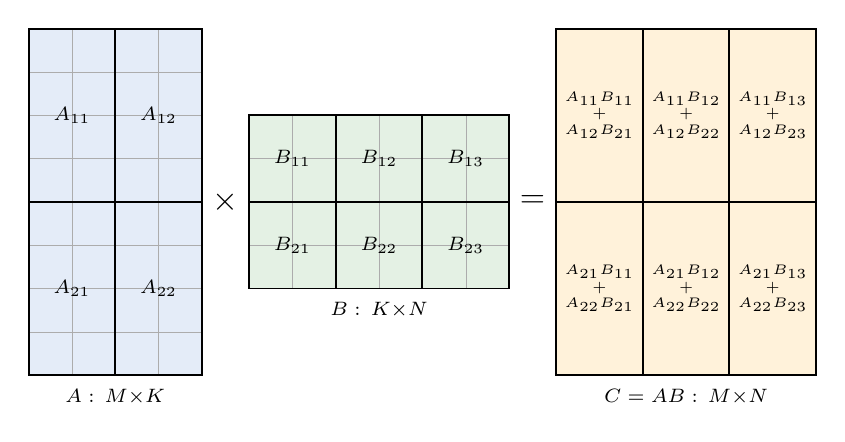
\begin{tikzpicture}[
    font=\tiny,
    cell/.style={draw=fagray!50, line width=0.1pt},
    block/.style={draw=black, line width=0.7pt},
  ]
    \def\sa{0.55}  % cell size in cm (uniform scale for A, B, and C)

    % --- Matrix A: 8x4 elements, 2x2 blocks (each block 4x2 cells) ---
    \begin{scope}[shift={(0, 0)}]
      \foreach \i in {0,...,7} \foreach \j in {0,...,3} {
        \draw[cell, fill=fablue!12]
          (\j*\sa, 7*\sa - \i*\sa) rectangle (\j*\sa + \sa, 8*\sa - \i*\sa);
      }
      \draw[block] (0, 0) rectangle (4*\sa, 8*\sa);
      \draw[block] (0, 4*\sa) -- (4*\sa, 4*\sa);
      \draw[block] (2*\sa, 0) -- (2*\sa, 8*\sa);
      \node[font=\scriptsize] at (1*\sa, 6*\sa) {$A_{11}$};
      \node[font=\scriptsize] at (3*\sa, 6*\sa) {$A_{12}$};
      \node[font=\scriptsize] at (1*\sa, 2*\sa) {$A_{21}$};
      \node[font=\scriptsize] at (3*\sa, 2*\sa) {$A_{22}$};
      \node[anchor=north, font=\scriptsize] at (2*\sa, -0.05) {$A:\, M{\times}K$};
    \end{scope}

    \node[font=\large] at (4*\sa + 0.3, 4*\sa) {$\times$};

    % --- Matrix B: 4x6 elements, 2x3 blocks (each block 2x2 cells) ---
    \begin{scope}[shift={(4*\sa + 0.6, 2*\sa)}]
      \foreach \i in {0,...,3} \foreach \j in {0,...,5} {
        \draw[cell, fill=fagreen!12]
          (\j*\sa, 3*\sa - \i*\sa) rectangle (\j*\sa + \sa, 4*\sa - \i*\sa);
      }
      \draw[block] (0, 0) rectangle (6*\sa, 4*\sa);
      \draw[block] (0, 2*\sa) -- (6*\sa, 2*\sa);
      \foreach \k in {1,2} {
        \draw[block] (2*\k*\sa, 0) -- (2*\k*\sa, 4*\sa);
      }
      \foreach \kc/\bj in {0/1, 1/2, 2/3} {
        \pgfmathsetmacro{\xc}{(2*\kc + 1)*\sa}
        \node[font=\scriptsize] at (\xc, 3*\sa) {$B_{1\bj}$};
        \node[font=\scriptsize] at (\xc, 1*\sa) {$B_{2\bj}$};
      }
      \node[anchor=north, font=\scriptsize] at (3*\sa, -0.05) {$B:\, K{\times}N$};
    \end{scope}

    \node[font=\large] at (4*\sa + 0.6 + 6*\sa + 0.3, 4*\sa) {$=$};

    % --- Matrix C: 2x3 grid of blocks. Each C block has the exact
    %     dimensions of (A block height) x (B block width) =
    %     (4 cells) x (2 cells) at the same \sa scale.
    \begin{scope}[shift={(4*\sa + 1.2 + 6*\sa, 0)}]
      \pgfmathsetmacro{\bw}{2*\sa}    % width  = 2 cells (= width of a B block)
      \pgfmathsetmacro{\bh}{4*\sa}    % height = 4 cells (= height of an A block)
      \foreach \i in {0,1} \foreach \j in {0,...,2} {
        \pgfmathtruncatemacro{\ii}{\i+1}
        \pgfmathtruncatemacro{\jj}{\j+1}
        \draw[block, fill=fasram!18]
          (\j*\bw, \bh - \i*\bh) rectangle (\j*\bw + \bw, 2*\bh - \i*\bh);
        \node[align=center, font=\tiny] at (\j*\bw + 0.5*\bw, 1.5*\bh - \i*\bh)
          {$A_{\ii 1}B_{1\jj}$\\$+$\\$A_{\ii 2}B_{2\jj}$};
      }
      \node[anchor=north, font=\scriptsize] at (1.5*\bw, -0.05) {$C = AB:\, M{\times}N$};
    \end{scope}
  \end{tikzpicture}
\end{frame}

\begin{frame}{Tiled Matrix Multiplication: The Idea}
\begin{columns}[T]
  \begin{column}{0.52\textwidth}
    \textbf{Naive matmul is bandwidth-bound:}
    \begin{itemize}\itemsep0.15em
      \item Every output element costs $2K$ global loads.
      \item Neighbouring threads re-fetch overlapping rows of $A$ and columns of $B$.
    \end{itemize}

    \vspace{0.4em}
    \textbf{Tiling idea:}
    \begin{itemize}\itemsep0.15em
      \item Partition $C$ into $T \times T$ output tiles.
      \item Assign \emph{one CUDA block per tile}; its $T^2$ threads cooperate.
      \item Walk $K$ in chunks of size $T$: at each step load one $A$-tile and one $B$-tile into \emph{shared memory}, then accumulate $A_t B_t$ into the $C$-tile.
    \end{itemize}

    \vspace{0.4em}
    \textbf{Why this wins:}
    \begin{itemize}\itemsep0.15em
      \item Each tile is loaded \emph{once}, reused $T$ times by every thread.
      \item Global loads per output: $2K \to 2K/T$ ($16\times$ drop for $T{=}16$).
      \item Shared memory is ${\sim}100\times$ faster than global.
    \end{itemize}
  \end{column}

  \begin{column}{0.48\textwidth}
    \centering
    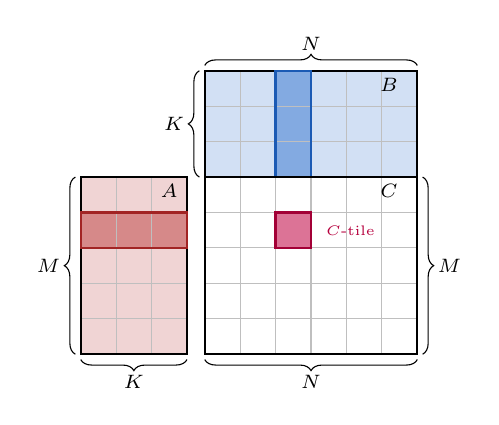
\begin{tikzpicture}[scale=0.45, font=\tiny]
      % --- B (top): K rows x N cols, partitioned ---
      \fill[fablue!20] (3.5, 5) rectangle (9.5, 8);
      \fill[fablue!55] (5.5, 5) rectangle (6.5, 8);
      \foreach \i in {4.5, 5.5, 6.5, 7.5, 8.5} { \draw[gray!50, thin] (\i, 5) -- (\i, 8); }
      \foreach \j in {6, 7} { \draw[gray!50, thin] (3.5, \j) -- (9.5, \j); }
      \draw[thick] (3.5, 5) rectangle (9.5, 8);
      \draw[thick, fablue!90!black] (5.5, 5) rectangle (6.5, 8);
      \node[font=\scriptsize] at (8.7, 7.6) {$B$};
      \draw[decorate, decoration={brace, amplitude=4pt}]
        (3.5, 8.15) -- (9.5, 8.15)
        node[midway, above=2pt, font=\scriptsize] {$N$};
      \draw[decorate, decoration={brace, amplitude=4pt}]
        (3.35, 5) -- (3.35, 8)
        node[midway, left=2pt, font=\scriptsize] {$K$};

      % --- A (left): M rows x K cols, partitioned ---
      \fill[fared!20] (0, 0) rectangle (3, 5);
      \fill[fared!55] (0, 3.0) rectangle (3, 4.0);
      \foreach \i in {1, 2} { \draw[gray!50, thin] (\i, 0) -- (\i, 5); }
      \foreach \j in {1, 2, 3, 4} { \draw[gray!50, thin] (0, \j) -- (3, \j); }
      \draw[thick] (0, 0) rectangle (3, 5);
      \draw[thick, fared!90!black] (0, 3.0) rectangle (3, 4.0);
      \node[font=\scriptsize] at (2.5, 4.6) {$A$};
      \draw[decorate, decoration={brace, amplitude=4pt}]
        (-0.15, 0) -- (-0.15, 5)
        node[midway, left=2pt, font=\scriptsize] {$M$};
      \draw[decorate, decoration={brace, amplitude=4pt, mirror}]
        (0, -0.15) -- (3, -0.15)
        node[midway, below=2pt, font=\scriptsize] {$K$};

      % --- C (bottom right): partitioned, one tile highlighted ---
      \foreach \i in {4.5, 5.5, 6.5, 7.5, 8.5} { \draw[gray!50, thin] (\i, 0) -- (\i, 5); }
      \foreach \j in {1, 2, 3, 4} { \draw[gray!50, thin] (3.5, \j) -- (9.5, \j); }
      \fill[purple!55] (5.5, 3.0) rectangle (6.5, 4.0);
      \draw[thick] (3.5, 0) rectangle (9.5, 5);
      \draw[thick, purple!85!black] (5.5, 3.0) rectangle (6.5, 4.0);
      \node[font=\scriptsize] at (8.7, 4.6) {$C$};
      \node[font=\tiny, purple!95!black, anchor=west] at (6.65, 3.5) {$C$-tile};
      \draw[decorate, decoration={brace, amplitude=4pt}]
        (9.65, 5) -- (9.65, 0)
        node[midway, right=2pt, font=\scriptsize] {$M$};
      \draw[decorate, decoration={brace, amplitude=4pt, mirror}]
        (3.5, -0.15) -- (9.5, -0.15)
        node[midway, below=2pt, font=\scriptsize] {$N$};
    \end{tikzpicture}

    \vspace{0.4em}
    {\scriptsize One $C$-tile is built from a row stripe of $A$ and a column stripe of $B$, walked in chunks of $T$ along the $K$ axis.}
  \end{column}
\end{columns}
\end{frame}

\newcommand{\tilestep}[1]{%
  \begin{tikzpicture}[scale=0.42, font=\tiny]
    \def\T{0.7}
    % --- Matrix B ---
    \begin{scope}[shift={(4*\T + 0.4, 3*\T + 0.4)}]
      \fill[fablue!20] (\T, 0) rectangle (2*\T, 4*\T);
      \fill[fablue!60] (\T, {(3-#1)*\T}) rectangle (2*\T, {(4-#1)*\T});
      \draw[thick] (0, 0) rectangle (3*\T, 4*\T);
      \foreach \i in {1,2} { \draw[gray!50, thin] (\i*\T, 0) -- (\i*\T, 4*\T); }
      \foreach \i in {1,2,3} { \draw[gray!50, thin] (0, \i*\T) -- (3*\T, \i*\T); }
      \draw[thick, fablue!90!black] (\T, {(3-#1)*\T}) rectangle (2*\T, {(4-#1)*\T});
      \node[above, font=\scriptsize] at (1.5*\T, 4*\T) {$B$};
      \node[font=\tiny, fablue!95!black] at (1.5*\T, {(3.5-#1)*\T}) {$B_{#1}$};
    \end{scope}
    % --- Matrix A ---
    \fill[fared!20] (0, \T) rectangle (4*\T, 2*\T);
    \fill[fared!60] ({#1*\T}, \T) rectangle ({(#1+1)*\T}, 2*\T);
    \draw[thick] (0, 0) rectangle (4*\T, 3*\T);
    \foreach \i in {1,2,3} { \draw[gray!50, thin] (\i*\T, 0) -- (\i*\T, 3*\T); }
    \foreach \i in {1,2} { \draw[gray!50, thin] (0, \i*\T) -- (4*\T, \i*\T); }
    \draw[thick, fared!90!black] ({#1*\T}, \T) rectangle ({(#1+1)*\T}, 2*\T);
    \node[above, font=\scriptsize] at (2*\T, 3*\T) {$A$};
    \node[font=\tiny, fared!95!black] at ({(#1+0.5)*\T}, 1.5*\T) {$A_{#1}$};
    % --- Matrix C ---
    \begin{scope}[shift={(4*\T + 0.4, 0)}]
      \draw[thick] (0, 0) rectangle (3*\T, 3*\T);
      \foreach \i in {1,2} { \draw[gray!50, thin] (\i*\T, 0) -- (\i*\T, 3*\T); }
      \foreach \i in {1,2} { \draw[gray!50, thin] (0, \i*\T) -- (3*\T, \i*\T); }
      \fill[purple!50] (\T, \T) rectangle (2*\T, 2*\T);
      \draw[thick, purple!80!black] (\T, \T) rectangle (2*\T, 2*\T);
      \node[right, font=\scriptsize] at (3*\T, 1.5*\T) {$C$};
      \node[font=\tiny, purple!95!black, align=center] at (1.5*\T, 1.5*\T) {$+\!\!=$\\$A_{#1} B_{#1}$};
    \end{scope}
    % --- Arrows ---
    \draw[->, thick, fared!90!black]
      ({(#1+1)*\T + 0.05}, 1.5*\T) -- (4*\T + 0.4 + \T - 0.05, 1.5*\T);
    \draw[->, thick, fablue!90!black]
      (4*\T + 0.4 + 1.5*\T, {3*\T + 0.4 + (3-#1)*\T - 0.05})
      -- (4*\T + 0.4 + 1.5*\T, 2*\T + 0.05);
  \end{tikzpicture}%
}

\begin{frame}{Tiled Matmul: Step by Step}
  \begin{columns}[T]
    \begin{column}{0.24\textwidth}
      \centering
      \tilestep{0}\\[0.2em]
      {\scriptsize Step $t = 0$}
    \end{column}
    \begin{column}{0.24\textwidth}
      \centering
      \tilestep{1}\\[0.2em]
      {\scriptsize Step $t = 1$}
    \end{column}
    \begin{column}{0.24\textwidth}
      \centering
      \tilestep{2}\\[0.2em]
      {\scriptsize Step $t = 2$}
    \end{column}
    \begin{column}{0.24\textwidth}
      \centering
      \tilestep{3}\\[0.2em]
      {\scriptsize Step $t = 3$}
    \end{column}
  \end{columns}

  \vspace{0.6em}
  {\small One block walks $K$ in chunks of $\mathtt{TILE}$. At each step $t$ it loads one $A$-tile $A_t$ and one $B$-tile $B_t$ into shared memory, then accumulates $A_t B_t$ into its $C$-tile.}
\end{frame}

\begin{frame}[fragile]{Tiled Matmul in CUDA: Walkthrough}
\begin{columns}[T]
  \begin{column}{0.58\textwidth}
\begin{lstlisting}[language=C++, keywordstyle=\color{fablue}\bfseries, basicstyle=\ttfamily\tiny, commentstyle=\color{fagreen!60!black}\itshape]
#define TILE 16
__global__ void cuda_matmul_tiled(float *C, float *A, float *B,
                                  int M, int N, int K)
{
    // (1) Setup
    __shared__ float As[TILE][TILE], Bs[TILE][TILE];
    int row = blockIdx.y * TILE + threadIdx.y;
    int col = blockIdx.x * TILE + threadIdx.x;
    float sum = 0.0f;

    // (2) Tile loop: walk K in chunks of TILE
    for (int t = 0; t < (K + TILE - 1) / TILE; ++t) {
        // (2a) Cooperative load of one tile pair
        As[threadIdx.y][threadIdx.x] =
            (row < M && t*TILE + threadIdx.x < K)
              ? A[row*K + t*TILE + threadIdx.x] : 0.0f;
        Bs[threadIdx.y][threadIdx.x] =
            (col < N && t*TILE + threadIdx.y < K)
              ? B[(t*TILE + threadIdx.y)*N + col] : 0.0f;
        __syncthreads();

        // (2b) Multiply-accumulate from shared mem
        for (int k = 0; k < TILE; ++k)
            sum += As[threadIdx.y][k] * Bs[k][threadIdx.x];
        __syncthreads();
    }
    // (3) Write-back
    if (row < M && col < N) C[row*N + col] = sum;
}
\end{lstlisting}
  \end{column}

  \begin{column}{0.42\textwidth}
    {\scriptsize
    \textbf{(1) Setup.}
    \begin{itemize}\itemsep0.1em
      \item \texttt{\_\_shared\_\_} declares per-block shared memory: visible to all $T^2$ threads in the block.
      \item \texttt{row, col}: this thread's output coordinate in $C$.
      \item \texttt{sum}: register-resident accumulator (private to the thread).
    \end{itemize}

    \vspace{0.4em}
    \textbf{(2a) Cooperative load.}
    \begin{itemize}\itemsep0.1em
      \item Each thread fetches \emph{one} element of $A_s$ and one of $B_s$; the $T^2$ threads together pull a full $T \times T$ tile pair.
      \item Boundary check pads with $0$ at the matrix edge.
      \item First \texttt{\_\_syncthreads()}: wait until every load lands before anyone reads.
    \end{itemize}

    \vspace{0.4em}
    \textbf{(2b) Multiply\textendash{}accumulate.}
    \begin{itemize}\itemsep0.1em
      \item Inner loop reads a row of $A_s$ and a column of $B_s$ from shared memory.
      \item Each shared-memory value is reused by $T$ threads $\Rightarrow$ global loads per output drop from $2K$ to $2K/T$.
      \item Second \texttt{\_\_syncthreads()}: stop fast threads from overwriting $A_s, B_s$ while others still read them.
    \end{itemize}

    \vspace{0.4em}
    \textbf{(3) Write-back.} One guarded global store per thread.
    }
  \end{column}
\end{columns}
\end{frame}

\begin{frame}{Triton: A Higher-Level GPU Language}
  \begin{itemize}
    \item \textbf{Triton} \cite{tillet2019triton} is a \textbf{Python-embedded DSL} for writing GPU kernels.
    \item You import \texttt{triton} and \texttt{triton.language as tl}, decorate a normal Python function with \texttt{@triton.jit}, and Triton compiles it to PTX/SASS at the first call.
    \item Originally from OpenAI; now widely used: PyTorch's \texttt{torch.compile} emits Triton kernels, FlashAttention has Triton implementations, etc.
    \item Goal: \emph{CUDA-like control with much less boilerplate}. You still pick block sizes and reason about memory, but you do not manage threads, shared memory, or synchronization by hand.
  \end{itemize}

  \vspace{0.5em}
  \begin{center}
  {\small
  \begin{tabular}{lll}
    \toprule
    \textbf{Concept} & \textbf{CUDA} & \textbf{Triton} \\
    \midrule
    Parallelism unit & Thread & Program (block-level) \\
    Memory access & Per-element load/store & Block load/store with masks \\
    Shared memory & Manual management & Automatic \\
    Synchronization & \texttt{\_\_syncthreads()} & Implicit \\
    Indexing & Scalar \texttt{threadIdx} arithmetic & Vectorized \texttt{tl.arange} \\
    \bottomrule
  \end{tabular}
  }
  \end{center}
\end{frame}

\begin{frame}{Triton: Core API}
  Most Triton kernels are built from a small set of block-level operations.

  \vspace{0.3em}
  \begin{center}
  {\scriptsize
  \begin{tabular}{lll}
    \toprule
    \textbf{Operation} & \textbf{Signature} & \textbf{Purpose} \\
    \midrule
    \multicolumn{3}{l}{\textit{Indexing \& launch}} \\
    \texttt{program\_id} & \texttt{tl.program\_id(axis)} & ID of current program along an axis \\
    \texttt{arange} & \texttt{tl.arange(start, end)} & Compile-time index vector $[\text{start}, \text{end})$ \\
    \texttt{constexpr} & \texttt{BLOCK: tl.constexpr} & Compile-time constant (enables specialization) \\
    \midrule
    \multicolumn{3}{l}{\textit{Memory}} \\
    \texttt{load} & \texttt{tl.load(ptr, mask, other)} & Block load with bounds mask \\
    \texttt{store} & \texttt{tl.store(ptr, val, mask)} & Block store with bounds mask \\
    \midrule
    \multicolumn{3}{l}{\textit{Compute}} \\
    \texttt{dot} & \texttt{tl.dot(a, b)} & Block matmul (uses tensor cores) \\
    \texttt{sum, max, min} & \texttt{tl.sum(x, axis)} & Block-level reductions \\
    \texttt{exp, log, sqrt} & \texttt{tl.exp(x)} & Elementwise math, vectorized \\
    \texttt{where} & \texttt{tl.where(cond, a, b)} & Elementwise select \\
    \midrule
    \multicolumn{3}{l}{\textit{Shapes}} \\
    \texttt{reshape} & \texttt{tl.reshape(x, shape)} & Reshape a block tensor \\
    \texttt{broadcast\_to} & \texttt{tl.broadcast\_to(x, shp)} & Explicit broadcast (NumPy-style auto bcast also works) \\
    \bottomrule
  \end{tabular}
  }
  \end{center}

  \vspace{0.3em}
  {\small
  \begin{itemize}
    \item \textbf{Block tensors:} small multidimensional arrays of compile-time fixed shape. They live in registers (not HBM); the user manipulates them as a single object, while the compiler implicitly spreads elements across the threads of the program.
    \item \textbf{NumPy-like semantics:} \texttt{tl.arange(0, BLOCK)} produces an index vector; broadcasting follows NumPy rules (e.g.\ \texttt{(BLOCK\_M, 1) * (1, BLOCK\_N) $\to$ (BLOCK\_M, BLOCK\_N)}); reductions \texttt{tl.sum}, \texttt{tl.max}, \texttt{tl.dot} act on whole blocks.
    \item \textbf{Pointers as block tensors:} \texttt{x\_ptr + tl.arange(0, BLOCK)} is itself a block tensor of pointers; \texttt{tl.load} on it fetches the whole block in one instruction.
    \item \textbf{Masks:} a boolean block tensor passed to \texttt{tl.load} / \texttt{tl.store} guards out-of-bounds elements; the compiler emits predicated loads.
    \item Triton handles vectorization, memory coalescing, and shared-memory staging behind the scenes; \texttt{tl.constexpr} parameters drive autotuning over \texttt{BLOCK\_SIZE}, \texttt{num\_warps}, \texttt{num\_stages}.
  \end{itemize}
  }
\end{frame}

\begin{frame}[fragile]{Triton Example: Vector Addition}
\begin{columns}[T]
  \begin{column}{0.55\textwidth}
\begin{lstlisting}[basicstyle=\ttfamily\scriptsize]
@triton.jit
def add_kernel(x_ptr, y_ptr, output_ptr,
               n_elements,
               BLOCK_SIZE: tl.constexpr):
    pid = tl.program_id(0)
    block_start = pid * BLOCK_SIZE
    offsets = block_start + tl.arange(0, BLOCK_SIZE)
    mask = offsets < n_elements
    x = tl.load(x_ptr + offsets, mask=mask)
    y = tl.load(y_ptr + offsets, mask=mask)
    tl.store(output_ptr + offsets, x + y, mask=mask)

# Launch
grid = lambda meta:
    (triton.cdiv(n, meta['BLOCK_SIZE']),)
add_kernel[grid](x, y, output, n,
                 BLOCK_SIZE=256)
\end{lstlisting}
  \end{column}
  \begin{column}{0.45\textwidth}
    \centering
    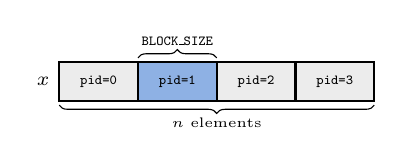
\begin{tikzpicture}[font=\tiny]
      \def\bw{1.0}
      \def\bh{0.5}
      \foreach \i/\fc in {0/gray!15, 1/fablue!50, 2/gray!15, 3/gray!15} {
        \fill[\fc] (\i*\bw, 0) rectangle ({(\i+1)*\bw}, \bh);
        \draw[thick] (\i*\bw, 0) rectangle ({(\i+1)*\bw}, \bh);
        \node[font=\tiny] at ({(\i+0.5)*\bw}, 0.5*\bh) {\texttt{pid=\i}};
      }
      % BLOCK_SIZE brace above block 1
      \draw[decorate, decoration={brace, amplitude=3pt}]
        (\bw, \bh + 0.05) -- (2*\bw, \bh + 0.05)
        node[midway, above=1pt, font=\tiny] {\texttt{BLOCK\_SIZE}};
      % n elements brace below
      \draw[decorate, decoration={brace, amplitude=3pt, mirror}]
        (0, -0.05) -- (4*\bw, -0.05)
        node[midway, below=1pt, font=\tiny] {$n$ elements};
      \node[left, font=\scriptsize] at (0, 0.5*\bh) {$x$};
    \end{tikzpicture}

    \vspace{0.6em}
    {\scriptsize
    \begin{itemize}\itemsep0.2em
      \item Vector partitioned into blocks of \texttt{BLOCK\_SIZE}; one Triton program per block.
      \item \texttt{pid = tl.program\_id(0)} identifies the current block.
      \item \texttt{offsets = pid*BLOCK\_SIZE + tl.arange(0, BLOCK\_SIZE)} is a length-\texttt{BLOCK\_SIZE} vector of element indices.
      \item Boolean \texttt{mask = offsets < n\_elements} disables out-of-range lanes in the tail block.
      \item \texttt{tl.load}/\texttt{tl.store} do masked block-level memory access.
    \end{itemize}
    }
  \end{column}
\end{columns}
\end{frame}

\begin{frame}[fragile]{Triton Example: Matrix Addition}
\begin{columns}[T]
  \begin{column}{0.5\textwidth}
\begin{lstlisting}[basicstyle=\ttfamily\scriptsize]
@triton.jit
def mat_add_kernel(A, B, C, M, N,
                   BLOCK_M: tl.constexpr,
                   BLOCK_N: tl.constexpr):
    pid_m = tl.program_id(0)
    pid_n = tl.program_id(1)
    offs_m = pid_m*BLOCK_M + tl.arange(0, BLOCK_M)
    offs_n = pid_n*BLOCK_N + tl.arange(0, BLOCK_N)
    mask = (offs_m[:, None] < M) \
         & (offs_n[None, :] < N)
    ptrs = offs_m[:, None]*N + offs_n[None, :]
    a = tl.load(A + ptrs, mask=mask)
    b = tl.load(B + ptrs, mask=mask)
    tl.store(C + ptrs, a + b, mask=mask)

# 2D grid launch
grid = lambda meta: (triton.cdiv(M, meta['BLOCK_M']),
                     triton.cdiv(N, meta['BLOCK_N']))
\end{lstlisting}

  \vspace{0.3em}
  {\scriptsize
  Concrete example: $M{=}N{=}8$, $\texttt{B\_M}{=}\texttt{B\_N}{=}4$, $(\texttt{pid\_m},\texttt{pid\_n}){=}(1,1)$, so
  $\texttt{offs\_m} = \texttt{offs\_n} = [4,5,6,7]$.
  }
  \end{column}
  \begin{column}{0.5\textwidth}
    \centering
    % Macro view: 3x3 grid of program-blocks
    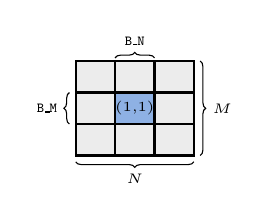
\begin{tikzpicture}[font=\tiny]
      \def\bw{0.5}
      \def\bh{0.4}
      \foreach \i in {0,1,2} {
        \foreach \j in {0,1,2} {
          \fill[gray!15] ({\i*\bw}, {(2-\j)*\bh}) rectangle ({(\i+1)*\bw}, {(3-\j)*\bh});
          \draw[thick] ({\i*\bw}, {(2-\j)*\bh}) rectangle ({(\i+1)*\bw}, {(3-\j)*\bh});
        }
      }
      \fill[fablue!50] (\bw, \bh) rectangle (2*\bw, 2*\bh);
      \draw[thick] (\bw, \bh) rectangle (2*\bw, 2*\bh);
      \node[font=\tiny] at (1.5*\bw, 1.5*\bh) {(1,1)};
      \draw[decorate, decoration={brace, amplitude=2pt}]
        (-0.08, \bh) -- (-0.08, 2*\bh)
        node[midway, left=1pt, font=\tiny] {\texttt{B\_M}};
      \draw[decorate, decoration={brace, amplitude=2pt}]
        (\bw, 3*\bh + 0.04) -- (2*\bw, 3*\bh + 0.04)
        node[midway, above=1pt, font=\tiny] {\texttt{B\_N}};
      \draw[decorate, decoration={brace, amplitude=2pt}]
        (3*\bw + 0.08, 3*\bh) -- (3*\bw + 0.08, 0)
        node[midway, right=1pt, font=\tiny] {$M$};
      \draw[decorate, decoration={brace, amplitude=2pt, mirror}]
        (0, -0.08) -- (3*\bw, -0.08)
        node[midway, below=1pt, font=\tiny] {$N$};
    \end{tikzpicture}

    \vspace{0.6em}
    % Micro view: offs_m, offs_n, ptrs block for (1,1)
    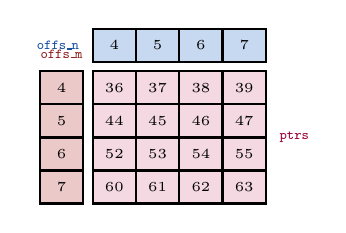
\begin{tikzpicture}[font=\tiny]
      \def\cw{0.55}
      \def\ch{0.42}
      \def\gap{0.12}

      % offs_n row at top
      \begin{scope}[shift={(0, 4*\ch + \gap)}]
        \foreach \v/\i in {4/0, 5/1, 6/2, 7/3} {
          \fill[fablue!25] ({\i*\cw}, 0) rectangle ({(\i+1)*\cw}, \ch);
          \draw[thick] ({\i*\cw}, 0) rectangle ({(\i+1)*\cw}, \ch);
          \node at ({(\i+0.5)*\cw}, 0.5*\ch) {\v};
        }
        \node[left, fablue!80!black, font=\tiny] at (-0.05, 0.5*\ch) {\texttt{offs\_n}};
      \end{scope}

      % offs_m column on left
      \begin{scope}[shift={(-\cw - \gap, 0)}]
        \foreach \v/\j in {4/0, 5/1, 6/2, 7/3} {
          \fill[fared!25] (0, {(3-\j)*\ch}) rectangle (\cw, {(4-\j)*\ch});
          \draw[thick] (0, {(3-\j)*\ch}) rectangle (\cw, {(4-\j)*\ch});
          \node at (0.5*\cw, {(3.5-\j)*\ch}) {\v};
        }
        \node[above, fared!80!black, font=\tiny] at (0.5*\cw, 4*\ch + 0.04) {\texttt{offs\_m}};
      \end{scope}

      % 4x4 ptrs block: ptrs[j][i] = offs_m[j]*N + offs_n[i] with N=8
      \foreach \i/\n in {0/4, 1/5, 2/6, 3/7} {
        \foreach \j/\m in {0/4, 1/5, 2/6, 3/7} {
          \pgfmathtruncatemacro{\ptr}{\m * 8 + \n}
          \fill[purple!15] ({\i*\cw}, {(3-\j)*\ch}) rectangle ({(\i+1)*\cw}, {(4-\j)*\ch});
          \draw[thick] ({\i*\cw}, {(3-\j)*\ch}) rectangle ({(\i+1)*\cw}, {(4-\j)*\ch});
          \node at ({(\i+0.5)*\cw}, {(3.5-\j)*\ch}) {\ptr};
        }
      }
      \node[right, purple!80!black, font=\tiny] at (4*\cw + 0.05, 2*\ch) {\texttt{ptrs}};
    \end{tikzpicture}

    \vspace{0.4em}
    {\scriptsize
    Broadcasting: $\texttt{ptrs}_{ji} = \texttt{offs\_m}_j \cdot N + \texttt{offs\_n}_i$.}
  \end{column}
\end{columns}
\end{frame}

\begin{frame}{Transpose via Strides}

  \textbf{Key trick:} Transposing a tensor only swaps its \emph{shape} and \emph{strides}. The physical memory is untouched, so the operation costs nothing.

  \vspace{0.6em}
  \centering
  \begin{tikzpicture}[
    font=\scriptsize,
    cell/.style={draw=fagray!70, minimum width=6mm, minimum height=6mm, inner sep=0pt, font=\scriptsize},
  ]
    % --- M: 3 cols x 2 rows, vertically centered around y=1.65 ---
    \node[font=\small] at (0.7, 2.85) {$M$};
    \foreach \i/\j/\v in {0/0/1, 0/1/2, 0/2/3, 1/0/5, 1/1/8, 1/2/13} {
      \node[cell, fill=fablue!20] at (\j*0.7, 2.0 - \i*0.7) {$\v$};
    }
    \node[font=\tiny, align=center, anchor=north] at (0.7, 0.55)
      {shape $[2,3]$\\stride $[3,1]$};

    % --- swap arrow between M and M^T ---
    \draw[->, very thick, fared] (1.85, 1.65) -- (3.15, 1.65);
    \node[font=\tiny, fared, anchor=south] at (2.5, 1.72) {swap strides};
    \node[font=\tiny, fared, anchor=north] at (2.5, 1.55) {(no copy)};

    % --- M^T: 2 cols x 3 rows, vertically centered around y=1.65 ---
    \node[font=\small] at (3.85, 2.85) {$M^\top$};
    \foreach \i/\j/\v in {0/0/1, 0/1/5, 1/0/2, 1/1/8, 2/0/3, 2/1/13} {
      \node[cell, fill=fasram!30] at (3.5 + \j*0.7, 2.35 - \i*0.7) {$\v$};
    }
    \node[font=\tiny, align=center, anchor=north] at (3.85, 0.55)
      {shape $[3,2]$\\stride $[1,3]$};

    % --- shared physical memory ---
    \node[font=\small] at (7.4, 2.85) {shared physical memory};
    \foreach \i/\v in {0/1, 1/2, 2/3, 3/5, 4/8, 5/13} {
      \node[cell, fill=fagreen!15] (p\i) at (5.3 + \i*0.7, 1.65) {$\v$};
    }
    \foreach \i/\addr in {0/62, 1/66, 2/70, 3/74, 4/78, 5/82} {
      \node[font=\tiny, fagray, below=-1pt of p\i] {\addr};
    }
    \node[font=\tiny, fagray, align=center, anchor=north] at (7.4, 0.95)
      {physical bytes \emph{unchanged}};
  \end{tikzpicture}

  \vspace{0.4em}
  \begin{itemize}\small
    \item Resulting view is non-contiguous: stride along the new fastest axis is no longer $1$
    \item Flash Attention uses this to load $K^\top$ for free by swapping the last two strides of $K$
  \end{itemize}
\end{frame}

\begin{frame}[fragile]{Transpose in Triton}
  Triton offers two ways to obtain a transposed tile, with very different cost:

  \textbf{(1) \texttt{tl.trans} -- explicit, moves data in registers / shared memory}
\begin{lstlisting}
X  = tl.load(X_ptr)                                # tile of shape [M, N]
XT = tl.trans(X)                                   # [N, M], physically rearranged
\end{lstlisting}
  Use when only a small tile already in registers needs to be flipped (e.g.\ \texttt{tl.trans(V\_block)} inside the FA backward to form $dP = dO\,V^\top$).

  \textbf{(2) Swap shape and strides in \texttt{tl.make\_block\_ptr} -- free}
\begin{lstlisting}
# Standard: load K as a [BLOCK_KV, HEAD_DIM] tile
K_ptr = tl.make_block_ptr(base=K, shape=(SEQ_LEN, HEAD_DIM),
                          strides=(stride_seq, stride_dim),
                          block_shape=(BLOCK_KV, HEAD_DIM), ...)

# Transposed: swap shape *and* strides -> tile loads as [HEAD_DIM, BLOCK_KV]
K_T_ptr = tl.make_block_ptr(base=K, shape=(HEAD_DIM, SEQ_LEN),
                            strides=(stride_dim, stride_seq),     # <-- swapped
                            block_shape=(HEAD_DIM, BLOCK_KV), ...)
K_T = tl.load(K_T_ptr)                             # equivalent to K^T, zero extra cost
\end{lstlisting}
  No data is moved: the block pointer simply walks the same physical memory along a different axis. This is exactly how Flash Attention's forward kernel gets $K^\top$ so that \texttt{tl.dot(Q\_block, K\_T)} computes $Q_i K_j^\top$ directly.

  \vspace{0.2em}
  {\footnotesize \textbf{Note:} A PyTorch-side \texttt{K.transpose(-2, -1)} before launching the kernel is also free (same stride trick) -- the kernel just sees pre-swapped strides.}
\end{frame}

% -----------------------------------------------------------------------
\subsection{Triton Implementation}

\begin{frame}[fragile]{Forward Kernel: Setup}
  Full \texttt{\_attn\_fwd} structure. Steps 1--3 construct the state that the
  inner loop (next slide) consumes; step 5 is the epilogue.

\begin{lstlisting}
@triton.jit
def _attn_fwd(Q, K, V, softmax_scale, M, O,
              stride_qb, stride_qh, stride_qs, stride_qd,             # strides of Q (K, V, O analogous)
              stride_kb, stride_kh, stride_ks, stride_kd,
              ..., NUM_HEADS, SEQ_LEN: tl.constexpr, HEAD_DIM: tl.constexpr,
              BLOCK_SIZE_Q: tl.constexpr, BLOCK_SIZE_KV: tl.constexpr, STAGE: tl.constexpr):

    # === 1. Which Q-block, which (batch, head) does this program own? ===
    block_index_q    = tl.program_id(0)
    index_batch_head = tl.program_id(1)
    qkv_offset       = index_batch_head * stride_qh                   # base offset for this (batch, head)

    # === 2. Block pointers.  Q and O are standard; K uses *swapped* strides. ===
    Q_block_ptr = tl.make_block_ptr(
        base=Q + qkv_offset, shape=(SEQ_LEN, HEAD_DIM),
        strides=(stride_qs, stride_qd),
        offsets=(block_index_q * BLOCK_SIZE_Q, 0),
        block_shape=(BLOCK_SIZE_Q, HEAD_DIM), order=(1, 0))

    # K viewed as [HEAD_DIM, SEQ_LEN]: shape AND strides swapped
    #   -> each tl.load yields K_j^T  (free transpose, no data movement)
    K_block_ptr = tl.make_block_ptr(
        base=K + qkv_offset, shape=(HEAD_DIM, SEQ_LEN),
        strides=(stride_kd, stride_ks),                               # <-- swapped vs. Q
        offsets=(0, 0),
        block_shape=(HEAD_DIM, BLOCK_SIZE_KV), order=(0, 1))

    V_block_ptr = tl.make_block_ptr(base=V + qkv_offset, ...,         # standard [BLOCK_KV, HEAD_DIM]
                                    block_shape=(BLOCK_SIZE_KV, HEAD_DIM))
    O_block_ptr = tl.make_block_ptr(base=O + qkv_offset, ...,         # standard [BLOCK_Q,  HEAD_DIM]
                                    block_shape=(BLOCK_SIZE_Q,  HEAD_DIM))

    # === 3. Load Q_i once into SRAM; init running state per row of Q_i ===
    Q_block = tl.load(Q_block_ptr)                                    # [BLOCK_Q, HEAD_DIM]
    m_i     = tl.zeros([BLOCK_SIZE_Q], tl.float32) - float("inf")     # running max
    l_i     = tl.zeros([BLOCK_SIZE_Q], tl.float32) + 1.0              # running sum
    O_block = tl.zeros([BLOCK_SIZE_Q, HEAD_DIM], tl.float32)          # output accumulator

    # === 4. Stream K, V blocks through SRAM and accumulate (see next slide) ===
    # Causal: call inner twice (STAGE=1 left of diag, STAGE=2 diag).  Non-causal: once.
    O_block, l_i, m_i = _attn_fwd_inner(O_block, l_i, m_i, Q_block,
                                         K_block_ptr, V_block_ptr,
                                         block_index_q, softmax_scale, STAGE, ...)

    # === 5. Epilogue: normalize O_i once; save L = m + log(l) for backward ===
    O_block = O_block / l_i[:, None]                                  # Trick 1
    m_i    += tl.math.log(l_i)                                        # Trick 2
    tl.store(O_block_ptr, O_block.to(O.type.element_ty))
    tl.store(M + index_batch_head * SEQ_LEN + offs_q, m_i)            # save log-sum-exp L
\end{lstlisting}

  \vspace{-0.3em}
  {\footnotesize Grid: \texttt{(ceil(SEQ\_LEN / BLOCK\_Q),\, BATCH$\cdot$HEADS,\, 1)} -- one program per $Q$-block per head.}
\end{frame}

\begin{frame}[fragile]{Forward: Streaming-Softmax Inner Loop}
  Body of \texttt{\_attn\_fwd\_inner}, invoked from \texttt{\_attn\_fwd} above. Each
  iteration streams one $K_j, V_j$ block from HBM; $Q_i$ and the running state
  $(m_i, \ell_i, O_i)$ stay resident in SRAM.

\begin{lstlisting}
# Stage selects which K, V range to scan (causal skips blocks fully right of diagonal)
if   STAGE == 1: lo, hi = 0, block_index_q * BLOCK_SIZE_Q                                # left of diag
elif STAGE == 2: lo, hi = block_index_q * BLOCK_SIZE_Q, (block_index_q+1)*BLOCK_SIZE_Q   # diagonal
else:            lo, hi = 0, SEQ_LEN                                                     # non-causal

K_block_ptr = tl.advance(K_block_ptr, (0, lo))                # K viewed as [HEAD_DIM, SEQ]
V_block_ptr = tl.advance(V_block_ptr, (lo, 0))                # V is        [SEQ, HEAD_DIM]

for start_kv in range(lo, hi, BLOCK_SIZE_KV):
    K_block  = tl.load(K_block_ptr)                           # K_j^T  [HEAD_DIM, BLOCK_KV]
    QK_block = tl.dot(Q_block, K_block)                       # S_ij = Q_i K_j^T  [BLOCK_Q, BLOCK_KV]

    # --- Online softmax: extend running max  m_i -> m_ij ---
    m_ij     = tl.maximum(m_i, tl.max(QK_block, 1) * softmax_scale)
    QK_block = QK_block * softmax_scale - m_ij[:, None]       # numerically safe shift
    P_block  = tl.math.exp(QK_block)                          # tilde P_ij
    l_ij     = tl.sum(P_block, 1)                             # rowsum(tilde P_ij)

    # --- Correction: rescale prior accumulators by alpha = exp(m_i - m_ij) ---
    alpha   = tl.math.exp(m_i - m_ij)
    l_i     = l_i * alpha + l_ij                              # l_i  <- alpha*l_i + rowsum
    O_block = O_block * alpha[:, None]                        # O_i  <- diag(alpha) O_i

    # --- Accumulate output: O_i += tilde P_ij V_j  (fused MAC into tl.dot) ---
    V_block = tl.load(V_block_ptr)                            # V_j   [BLOCK_KV, HEAD_DIM]
    O_block = tl.dot(P_block.to(tl.float16), V_block, O_block)

    m_i = m_ij
    K_block_ptr = tl.advance(K_block_ptr, (0, BLOCK_SIZE_KV))
    V_block_ptr = tl.advance(V_block_ptr, (BLOCK_SIZE_KV, 0))
\end{lstlisting}
\end{frame}

\begin{frame}[fragile]{Backward: Two-Phase Kernel}
  Two grid launches share the math but invert the outer loop. $P_{ij}$ is
  \emph{recomputed} from $Q,K$ and the saved log-sum-exp $L_i$;
  $D_i = \mathrm{rowsum}(dO_i \odot O_i)$ replaces materializing $dP$.

  \textbf{Phase 1 (outer loop over $Q$-blocks $\to$ accumulate $dQ_i$):}
\begin{lstlisting}
Q_block, dO_block = tl.load(Q_block_ptr), tl.load(dO_block_ptr)        # Q_i, dO_i
L_i = tl.load(M + offs_q)                                              # saved logsumexp
D_i = tl.sum(dO_block * tl.load(O_ptr), 1)                             # D_i = rowsum(dO * O)
dQ_block = tl.zeros([BLOCK_SIZE_Q, HEAD_DIM], tl.float32)
for start_kv in range(0, SEQ_LEN, BLOCK_SIZE_KV):
    K_block, V_block = tl.load(K_block_ptr), tl.load(V_block_ptr)
    P_block  = tl.math.exp(tl.dot(Q_block, K_block) * softmax_scale - L_i[:, None])  # recompute
    dP_block = tl.dot(dO_block, tl.trans(V_block))                     # dP = dO V^T
    dS_block = P_block * (dP_block - D_i[:, None])                     # dS = P * (dP - D)
    dQ_block += tl.dot(dS_block.to(tl.float16), tl.trans(K_block))     # dQ_i += dS K
tl.store(dQ_block_ptr, dQ_block.to(tl.float16))
\end{lstlisting}

  \textbf{Phase 2 (outer loop over $K,V$-blocks $\to$ accumulate $dK_j, dV_j$):}
\begin{lstlisting}
K_block, V_block = tl.load(K_block_ptr), tl.load(V_block_ptr)          # K_j, V_j stay resident
dK_block = tl.zeros([BLOCK_SIZE_KV, HEAD_DIM], tl.float32)
dV_block = tl.zeros([BLOCK_SIZE_KV, HEAD_DIM], tl.float32)
for start_q in range(0, SEQ_LEN, BLOCK_SIZE_Q):
    Q_block, dO_block = tl.load(Q_block_ptr), tl.load(dO_block_ptr)    # stream Q_i, dO_i
    L_i, D_i = tl.load(M + offs_q), tl.load(D_ptr + offs_q)
    # P now has rows=KV, cols=Q  (transposed view of phase 1)
    P_block  = tl.math.exp(tl.dot(K_block, tl.trans(Q_block)) * softmax_scale - L_i[None, :])
    dV_block += tl.dot(P_block, dO_block)                              # dV_j += P_ij^T dO_i
    dP_block  = tl.dot(V_block, tl.trans(dO_block))
    dS_block  = P_block * (dP_block - D_i[None, :])
    dK_block += tl.dot(dS_block, Q_block)                              # dK_j += dS_ij^T Q_i
\end{lstlisting}
\end{frame}

\begin{frame}[fragile]{PyTorch Autograd Wrapper}
  Glues the Triton kernels into PyTorch so attention is a normal differentiable op.

\begin{lstlisting}
class TritonAttention(torch.autograd.Function):
    @staticmethod
    def forward(ctx, Q, K, V, causal, softmax_scale):
        BATCH, HEADS, SEQ_LEN, HEAD_DIM = Q.shape
        O = torch.empty_like(Q)
        # M holds the per-row log-sum-exp L (fp32 -- needed by backward)
        M = torch.empty((BATCH, HEADS, SEQ_LEN), device=Q.device, dtype=torch.float32)
        grid = lambda a: (triton.cdiv(SEQ_LEN, a["BLOCK_SIZE_Q"]), BATCH*HEADS, 1)
        _attn_fwd[grid](Q, K, V, softmax_scale, M, O, ...,
                         STAGE=3 if causal else 1)         # STAGE selects causal vs. non-causal
        ctx.save_for_backward(Q, K, V, O, M)               # only fp16/bf16 tensors needed
        ctx.softmax_scale = softmax_scale
        return O

    @staticmethod
    def backward(ctx, dO):
        Q, K, V, O, M = ctx.saved_tensors                  # M = log-sum-exp L
        dQ, dK, dV = torch.empty_like(Q), torch.empty_like(K), torch.empty_like(V)
        _attn_bwd[grid](Q, K, V, ctx.softmax_scale, dO, dQ, dK, dV, M, ...)
        return dQ, dK, dV, None, None                      # None for causal, softmax_scale
\end{lstlisting}
\end{frame}

\begin{frame}{Causal vs.\ Non-Causal Attention}

  \begin{columns}
    \begin{column}{0.55\textwidth}
      \textbf{Causal (autoregressive) attention:}
      \begin{itemize}\itemsep1pt
        \item Token $i$ may attend only to tokens $j \leq i$
        \item Standard implementation computes full $S$, then masks the upper triangle: roughly half the work is wasted
        \item Flash Attention skips blocks fully above the diagonal entirely
      \end{itemize}

      \vspace{0.3em}
      \textbf{Three block categories per $Q_i$ row:}
      \begin{description}\itemsep1pt
        \item[Stage 1 (left of diag.)] All entries valid $\to$ no mask, fastest path
        \item[Stage 2 (on diag.)] Apply causal mask: $S_{i,j} \!\gets\! -\infty$ where $j > i$
        \item[Skipped (right of diag.)] Inner-loop bound \texttt{hi=block\_index\_q*BLOCK\_Q} stops short
      \end{description}

      \vspace{0.3em}
      \textbf{Consequences:}
      \begin{itemize}\itemsep1pt
        \item Causal FA is $\sim\!2\times$ faster than non-causal at long context
        \item Only one masked block per $Q$-row $\to$ small overhead
        \item Kernel runs the inner loop \emph{twice} (Stage 1, then Stage 2)
      \end{itemize}

      \vspace{0.3em}
      \textbf{Non-causal:} single inner-loop pass over the full sequence; no mask, no skipping.
    \end{column}
    \begin{column}{0.42\textwidth}
      \begin{center}
      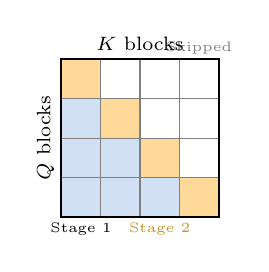
\begin{tikzpicture}[scale=0.5]
        \fill[fablue!20] (0,3) rectangle (1,4);
        \fill[fablue!20] (0,2) rectangle (2,3);
        \fill[fablue!20] (0,1) rectangle (3,2);
        \fill[fablue!20] (0,0) rectangle (4,1);
        \fill[fasram!50] (0,3) rectangle (1,4);
        \fill[fasram!50] (1,2) rectangle (2,3);
        \fill[fasram!50] (2,1) rectangle (3,2);
        \fill[fasram!50] (3,0) rectangle (4,1);
        \draw[step=1, gray, thin] (0,0) grid (4,4);
        \draw[thick] (0,0) rectangle (4,4);
        \node[font=\tiny] at (0.5, -0.3) {Stage 1};
        \node[font=\tiny, fasram!80!black] at (2.5, -0.3) {Stage 2};
        \node[font=\tiny, gray] at (3.5, 4.3) {Skipped};
        \node[font=\scriptsize, rotate=90] at (-0.4, 2) {$Q$ blocks};
        \node[font=\scriptsize] at (2, 4.4) {$K$ blocks};
      \end{tikzpicture}
      \end{center}
    \end{column}
  \end{columns}
\end{frame}

\begin{frame}{Flash Attention: Summary}

  \begin{enumerate}
    \item \textbf{Problem}: Standard attention is \emph{memory-bound} due to materializing $T \times T$ matrices in HBM
    \item \textbf{Solution}: Tile the computation, keep blocks in SRAM, use online softmax to avoid materializing the full attention matrix
    \item \textbf{Streaming softmax}: Enables incremental softmax computation across blocks with a running max and sum
    \item \textbf{Kernel fusion}: Single fused kernel for the entire forward pass. No intermediate HBM writes
    \item \textbf{Backward pass}: Recompute attention weights from $Q, K$ instead of storing them; use saved logsumexp $L$
    \item \textbf{Result}: Exact attention (not an approximation!) with $O(T)$ memory and significantly faster wall-clock time
  \end{enumerate}

  \vspace{0.5em}
  \begin{alertblock}{Impact}
    Flash Attention is now the default attention implementation in most deep learning frameworks and has enabled training with much longer context lengths.
    We will later discuss ring attention and tree attention for scaling to even larger contexts.
  \end{alertblock}
\end{frame}
